%\documentclass[preprint,12pt]{elsarticle}

%% Use the options 1p,twocolumn; 3p; 3p,twocolumn; 5p; or 5p,twocolumn
%% for a journal layout:
%%  \documentclass[final,1p,times]{elsarticle}
%% \documentclass[final,1p,times,twocolumn]{elsarticle}
%% \documentclass[final,3p,times]{elsarticle}
%% \documentclass[final,3p,times,twocolumn]{elsarticle}
%\documentclass[final,5p,times]{elsarticle}
\documentclass[final,5p,times,twocolumn]{elsarticle}

%% if you use PostScript figures in your article
%% use the graphics package for simple commands
%% \usepackage{graphics}
%% or use the graphicx package for more complicated commands
%% \usepackage{graphicx}
%% or use the epsfig package if you prefer to use the old commands
%% \usepackage{epsfig}

%% The amssymb package provides various useful mathematical symbols
\usepackage{amssymb}

\usepackage{makeidx}  % allows for indexgeneration
\usepackage{algorithm,algpseudocode}
\usepackage{graphicx}
\usepackage{float}
\usepackage{subcaption}
\captionsetup{compatibility=false}
\usepackage{wrapfig}
\usepackage{array}
%% \usepackage{cite}
% The amsthm package provides extended theorem environments
%% \usepackage{amsthm}

%% The lineno packages adds line numbers. Start line numbering with
%% \begin{linenumbers}, end it with \end{linenumbers}. Or switch it on
%% for the whole article with \linenumbers after \end{frontmatter}.
%% \usepackage{lineno}

%% natbib.sty is loaded by default. However, natbib options can be
%% provided with \biboptions{...} command. Following options are
%% valid:

%%   round  -  round parentheses are used (default)
%%   square -  square brackets are used   [option]
%%   curly  -  curly braces are used      {option}
%%   angle  -  angle brackets are used    <option>
%%   semicolon  -  multiple citations separated by semi-colon
%%   colon  - same as semicolon, an earlier confusion
%%   comma  -  separated by comma
%%   numbers-  selects numerical citations
%%   super  -  numerical citations as superscripts
%%   sort   -  sorts multiple citations according to order in ref. list
%%   sort&compress   -  like sort, but also compresses numerical citations
%%   compress - compresses without sorting
%%
%% \biboptions{comma,round}

% \biboptions{}
\journal{Future Generation of Computer Systems}

\begin{document}

\begin{frontmatter}

%% Title, authors and addresses

%% use the tnoteref command within \title for footnotes;
%% use the tnotetext command for the associated footnote;
%% use the fnref command within \author or \address for footnotes;
%% use the fntext command for the associated footnote;
%% use the corref command within \author for corresponding author footnotes;
%% use the cortext command for the associated footnote;
%% use the ead command for the email address,
%% and the form \ead[url] for the home page:
%%
\title{Quantitative and Structural Analysis in Scientific Workflows}

%% \title{Title\tnoteref{label1}}
%% \tnotetext[label1]{}
%% \author{Name\corref{cor1}\fnref{label2}}
%% \ead{email address}
%% \ead[url]{home page}
%% \fntext[label2]{}
%% \cortext[cor1]{}
%% \address{Address\fnref{label3}}
%% \fntext[label3]{}


\author[isi]{Weiwei Chen\corref{cor1}}
\ead{weiweich@acm.org}

\author[lyon]{Rafael Ferreira da Silva}
\ead{rafael.silva@creatis.insa-lyon.fr}

\author[isi]{Ewa Deelman}
\ead{deelman@isi.edu}



\author[man]{Rizos Sakellariou}
\ead{rizos@cs.man.ac.uk}

\cortext[cor1]{Corresponding address: USC Information Sciences Institute, 4676 Admiralty Way Ste 1001, Marina del Rey, CA, USA, 90292, Tel: +1 310 448-8408}


\address[isi]{University of Southern California, Information Sciences Institute,
		Marina del Rey, CA, USA}
\address[lyon]{University of Lyon, CNRS, Villeurbanne, France}
\address[man]{University of Manchester, School of Computer Science, Manchester, U.K.}


\begin{abstract}
Researchers working on the planning, scheduling, and execution of scientific workflows need access to a wide variety of scientific workflows to evaluate the performance of their implementations. This paper provides a characterization of workflows from six diverse scientific applications, including astronomy, bioinformatics, earthquake science, and gravitational-wave physics. The characterization is based on novel workflow profiling tools that provide detailed information about the various computational tasks that are present in the workflow. This information includes I/O, memory and computational characteristics. Although the workflows are diverse, there is evidence that each workflow has a job type that consumes the most amount of runtime. The study also uncovered inefficiency in a workflow component implementation, where the component was re-reading the same data multiple times.

Scientific workflow systems support various workflow representations, operational modes, and configurations. Regardless of the system used, end users have common needs: to track the status of their workflows in real time, be notified of execution anomalies and failures automatically, perform troubleshooting, and automate the analysis of the workflow results. In this paper, we describe how the Stampede monitoring
infrastructure was integrated with the Pegasus
Workflow Management System and the Triana
Workflow Systems, in order to add generic real

reveals internal features also the complexity is reduced. 
\end{abstract}

\begin{keyword}
%% keywords here, in the form: keyword \sep keyword

%% MSC codes here, in the form: \MSC code \sep code
%% or \MSC[2008] code \sep code (2000 is the default)
Scientific workflows \sep Log analysis \sep Workflow performance data \sep Workflow Simulation

\end{keyword}

\end{frontmatter}

\section{Introduction}
\label{intro}

move introduction of each session to the top session
%Basic introduction of workflows

Over the years, with the emerging of the fourth paradigm of science discovery \cite{Hey2009}, scientific workflows continue to gain their popularity among many science disciplines, including physics \cite{Deelman2002}, astronomy \cite{Sakellariou2010}, biology \cite{Lathers2006, Oinn2004}, chemistry \cite{Wieczorek2005}, earthquake science \cite{Maechling2007} and many more. Scientific workflows increasingly require tremendous amounts of data processing and workflows with up to a few million tasks are not uncommon \cite{Callaghan2011}. 
%workflow analysis tools

%We present a series and show how they promote a broad range of workflow related researches, including workflow profiling and characterizing, workflow balancing, and workflow scheduling

%Computational scientists are running increasingly complex, data-intensive simulations and analyses. Many scientific communities use workflow technologies to manage this complexity [1]. Workflow technologies are responsible for scheduling computational tasks on distributed resources, for managing dependencies among tasks, and for staging data sets into and out of execution sites. 
As scientific workflows grow in complexity and importance, the designers of workflow management systems 
need a deeper and broader understanding of what workflows require and how they behave in order to drive 
improvements in algorithms for provisioning resources, scheduling computational jobs, and managing data. To 
date, the community has lacked detailed a set of quantitative and structural analysis methodologies. Traditionally, there have been a plenty of work on workflow analysis based on intuition and experience. However, with the growth of the workflow scale, it is nearly impossible to apply these intuition to large scale workflows. Therefore, the increase of the amount of data processing requires a quantitative rather than imperical analysis tools. What is more, researchers are able to identify the workflow characteristics and features in a task level, such as resource requirement of a task. In many scientific applications, workflows are used to describe the relationships between individual computational components. However, with the complicated data dependencies within a workflow, we require a complete tool to analyze the internal structure of a workflow. By structural, we mean data dependencies and thus it is workflow level. By quantitative, we mean it is comparable and fit for general use. rather than case by case. 

We are also overhead aware and then the importance of overhead from thesis. 

They are also interested in a common set of performance metrics such as how long the workflow ran, how many jobs it had, the breakdown of jobs by various types, and compute resource usage. Even though they are numerical, they are still not quantitative because they are not comparable. In our case, we try to isolate the influence factors as much as possible. 

%In many scientific applications, workflows are used to describe the relationships between individual computational components [14]. Scientific workflows enable the formalization of the compu- tations, exposing individual computational steps, and data and control dependencies between them. They allow scientists to focus on the logical struc- ture of the overall computation rather than on the low-level implementation details. Representing the computation as a workflow makes updating and maintaining an application easier than mod- ifying a complex script that represents the same computation.

\section{Related Work}
%should fix it

In characterizing the execution profile for each workflow, we present such parameters as the number of 
jobs of each type and the I/O, memory, and CPU requirements of each job type. The workflows that we 
characterize are taken from diverse application domains such as astronomy, biology, gravitational physics and 
earthquake science. Together, they provide a broad overview of the types of applications that currently use 
workflow technologies to manage complex analyses. They also represent different types of workflows from small 
to large-scale, and include I/O-intensive, CPU-intensive, and memory-bound codes.
The goal of these workflow characterizations is to provide a community resource that will allow the designers 
and users of workflow systems to base their evaluation of algorithms and technologies on the characteristics of a 
broader range of workflows. These characterizations can be used by the research community even when application 
code and data are not available to develop synthetic workflows, benchmarks, and simulations for evaluating 
workflow managementsystems. 
Prior work [12, 13] has focused on workflow patterns and workflow system taxonomies, respectively. In this 
paper, we focus on workflow characterization from the point of view of the performance of the individual 
workflow components and overall workflows. The goal is to obtain detailed task-level performance metrics similar 
to those described in [14, 15]. In addition to being useful for understanding and simulating workflows to improve 
workflow management systems, this data has a number of other uses. Many existing workflow systems provide 
support for capturing provenance [16-18]. Profile data could be stored along with provenance to provide a more 
complete history of the execution of a workflow. The information could also be used to improve workflow 
scheduling. Many scheduling algorithms require runtime and data estimates in order to optimize workflow 
execution [19-22]. Profile data could be used to create a performance model of the workflow that is able to 
generate these estimates. Similarly, profile data could be used to guide resource provisioning algorithms that 
require estimates of resource usage [23-26].

%should fix it
Workflows present compact operational models of complex domain processes, which can assist substantially in the understanding and learning of these processes. A workflow can be used to systematically break up a complex problem into a tractable set of components that support the entire research lifecycle. It promotes a gen- eral methodology for disseminating good research practices and their reuse across institutions, prob- lem domains, and disciplines.
There are numerous workflow systems in use within the scientific community, for exam- ple, ASKALON [16], Kepler [3], Pegasus [12], MOTEUR [19], P-Grade [24], Taverna [28], Triana [22] and Trident [6]. Workflow standards such as the Business Process Execution Lan- guage (BPEL) [5, 29] have been applied to sci- entific problems [15]. However, there has not been much work in providing a common workflow monitoring tool within the eScience community. Instead, the community has focussed on achiev- ing interoperability at the workflow representa- tion level, which enables users to run the same workflow using different workflow engines or by embedding workflows as black box processes, e.g. SHIWA [47], WF4Ever [44]. The relative lack of common monitoring representations has led to development of higher-level analysis capabilities in disconnected “silos” for each work- flow tool, duplicating effort and slowing overall progress.
Many workflow systems have some form of integrated monitoring capability. For example, Kepler, Triana, and Taverna support runtime monitoring through a graphical user interface. Some systems, like P-GRADE [24], support inte- grated performance analysis and debugging. Al- though there is a common set of analysis needs across these workflow systems, there is little in- teroperability between the monitoring capabili- ties. To date, interoperability of workflow state information has been focused on the prove- nance of computations, e.g.: the IETF Open Provenance Model [45], OPM-V [46], PREMIS [31], and SWAN [39]. These provenance systems focus primarily on capturing the relationship between data and computations defined in a workflow rather than performance information. However, we leverage some of our prior prove- nance work [27] to capture the relationships between the user defined workflows and the work- flows actually executed by the workflow systems.
Most of these systems are focused on mon- itoring correctness and performance of the or- chestration and application, stopping short of coordination with monitoring of the computa- tional infrastructure. An exception is Condor’s Quill [23], which provides well-defined interfaces to operational data from the scheduling substrate. However, this operational data is geared towards providing a global view of the computational in- frastructure (i.e a Condor Pool). It is very difficult to correlate its statistics with the particular se- quences of activities in a given workflow, sub- workflow, job, and so on. There is no way to directly associate jobs in a particular workflow with the data in the Quill database. Quill can be used to see jobs running by a particular user. However, it does not help in identifying what higher level workflow it belongs to. Quill serves the needs of an administrator of a computational resource, whereas we are concerned with the user experience.

%balancing
The low performance of fine-grained tasks is a common problem in widely distributed platforms where the scheduling overhead and queuing times are high, such as Grid and Cloud systems. Several works have addressed the control of task granularity of bag of tasks. For instance, Muthuvelu et al. [3] proposed a clustering algorithm that groups bag of tasks based on their runtime—tasks are grouped up to the resource capacity. Later, they extended their work [4] to determine task granularity based on task file size, CPU time, and resource constraints. Recently, they proposed an online scheduling algorithm [5], [6] that groups tasks based on resource network utilization, user’s budget, and application deadline. Ng et al. [7] and Ang et al. [8] introduced bandwidth in the scheduling framework to enhance the performance of task scheduling. Longer tasks are assigned to resources with better bandwidth. Liu and Liao [9] proposed an adaptive fine- grained job scheduling algorithm to group fine-grained tasks according to processing capacity and bandwidth of the current available resources. Although these techniques significantly reduce the impact of scheduling and queuing time overhead, they are not applicable to scientific workflows, since data dependencies are not considered.
Task granularity control has also been addressed in scientific workflows. For instance, Singh et al. [10] proposed a level- and label-based clustering. In level-based clustering, tasks at the same level can be clustered together. The number of clusters or tasks per cluster are specified by the user. In the label-based clustering, the user labels tasks that should be clustered together. Although their work considers data dependency between workflow levels, it is done manually by users, which is prone to errors. Recently, Ferreira da Silva et al. [11] proposed task grouping and de-grouping algorithms to control workflow task granularity in a non-clairvoyant and online context. Their work significantly reduced scheduling and queuing time overheads, but did not consider data depen- dencies.
A plethora of balanced scheduling algorithms have been developed in the networking and OS domains. Many of these schedulers have been extended to the hierarchical setting. Lifflander et al. [12] proposed to use work stealing and a hierarchical persistence-based rebalancing algorithm to address the imbalance problem in scheduling. Zheng et al. [14] pre- sented an automatic hierarchical load balancing method that overcomes the scalability challenges of centralized schemes and poor solutions of traditional distributed schemas. There are other scheduling algorithms [15] (e.g. list scheduling)
that indirectly achieve load balancing of workflows through makespan minimization. However, the benefit that can be achieved through traditional scheduling optimization is limited by its complexity. The performance gain of task clustering is primarily determined by the ratio between system overheads and task runtime, which is more substantial in modern dis- tributed systems such as Clouds and Grids.

%should fix it
We now briefly describe the scientific workflows that we have characterized.Montage: Montage [2] was created by the NASA/IPAC Infrared Science Archive as an open source toolkit that 
can be used to generate custom mosaics of the sky using input images in the Flexible Image Transport System 
(FITS) format. During the production of the final mosaic, the geometry of the output image is calculated from the 
input images. The inputs are then re-projected to have the same spatial scale and rotation, the background 
emissions in the images are corrected to have a uniform level, and the re-projected, corrected images are co-added 
to form the output mosaic. The Montage application has been represented as a workflow that can be executed in 
Grid environments such as the TeraGrid [30].
CyberShake: The CyberShake workflow [31] is used by the Southern California Earthquake Center (SCEC)
[32] to characterize earthquake hazards using the Probabilistic Seismic Hazard Analysis (PSHA) technique. Given 
a region of interest, an MPI based finite difference simulation is performed to generate Strain Green Tensors 
(SGTs). From the SGT data, synthetic seismograms are calculated for each of a series of predicted ruptures. Once 
this is done, spectral acceleration and probabilistic hazard curves are calculated from the seismograms to 
characterize the seismic hazard. CyberShake workflows composed of more than 800,000 jobs have been executed 
using the Pegasus workflow management system on the TeraGrid [33, 34].
Broadband: Broadband is a computational platform used by the Southern California Earthquake Center [32]. 
The objective of Broadband is to integrate a collection of motion simulation codes and calculations to produce 
research results of value to earthquake engineers. These codes are composed into a workflow that simulates the 
impact of one or more earthquakes on one of several recording stations. Researchers can use the Broadband 
platform to combine low frequency (less than 1.0Hz) deterministic seismograms with high frequency (∼10Hz) 
stochastic seismograms and calculate various ground motion intensity measures (spectral acceleration, peak ground 
acceleration and peak ground velocity) for building design analysis.
Epigenomics: The USC Epigenome Center [35] is currently involved in mapping the epigenetic state of human 
cells on a genome-wide scale. The Epigenomics workflow is essentially a data processing pipeline that uses the 
Pegasus workflow management system to automate the execution of the various genome sequencing operations. 
DNA sequence data generated by the Illumina-Solexa [36] Genetic Analyzer system is split into several chunks 
that can be operated on in parallel. The data in each chunk is converted into a file format that can be used by the 
Maq software that maps short DNA sequencing reads [37, 38]. From there, the sequences are filtered to remove 
noisy and contaminating segments and mapped into the correct location in a reference genome, Finally, a global 
map of the aligned sequences is generated and the sequence density at each position in the genome is calculated. 
This workflow is being used by the Epigenome Center in the processing of production DNA methylation and 
histone modification data.
LIGO Inspiral Analysis: The Laser Interferometer Gravitational Wave Observatory (LIGO) [39, 40] is 
attempting to detect gravitational waves produced by various events in the universe as per Einstein’s theory of 
general relativity. The LIGO Inspiral Analysis workflow [41] is used to analyze the data obtained from the coalescing of compact binary systems such as binary neutron stars and black holes. The time-frequency data from 
each of the three LIGO detectors is split into smaller blocks for analysis. For each block, the workflow generates a 
subset of waveforms belonging to the parameter space and computes the matched filter output. If a true inspiral has 
been detected, a trigger is generated that can be checked with triggers for the other detectors. Several additional 
consistency tests may also be added to the workflow.
SIPHT: The bioinformatics project at Harvard University is conducting a wide search for small, untranslated 
RNAs (sRNAs) that regulate processes such as secretion and virulence in bacteria. The sRNA Identification 
Protocol using High-throughput Technology (SIPHT) program [42] uses a workflow to automate the search for 
sRNA encoding-genes for all bacterial replicons in the National Center for Biotechnology Information (NCBI) 
database. The kingdom-wide prediction and annotation of sRNA encoding genes involves a variety of programs 
that are executed in the proper order using Condor DAGMan’s [43, 44] capabilities. These involve the prediction 
of Rho-independent transcriptional terminators, BLAST (Basic Local Alignment Search Tools) comparisons of the 
inter-genetic regions of different replicons and the annotations of any sRNAs that are found.


%Stamepe 
Most workflow systems have addressed this need by building their own specific monitoring in- frastructure [30] or by putting logs into a database
post mortem and then performing the analysis [8]. These approaches duplicate effort that could be more efficiently combined to build a common analysis infrastructure.
A system that attempts to address these con- cerns and provide a common data model for filtering monitoring information across runs is the NSF-funded Synthesized Tools for Archiving Monitoring Performance and Enhanced DEbug- ging (Stampede) [21, 37] project. In this project, the authors have developed a framework that uses a general data model to represent workflows and their execution. Stampede decouples the repre- sentation of data in the workflow and job log files from the process of populating this data to a cen- tral store. This decoupling provides the potential to use the Stampede framework for loading logs and analysis across workflow systems.
In previous work [50] we have described the basic features of the Stampede data model and shown its integration with Triana. The contributions of the present paper are:

Stampede data model. Stampede is a complete workflow data model for repre- senting the performance characteristics of distributed workflows. It can track workflow restructuring employed by workflow systems at runtime. This allows queries that reference the workflow originally defined by the user to be answered using data collected during execution.
– Data model generality. The paper demon- strates the applicability of the Stampede model to scientific workflow systems in gen- eral by showing the integration of Stampede with two independent and different workflow systems, Pegasus WMS and Triana.
– Analysis capabilities. The Stampede data model provides a common and more powerful platform for troubleshooting and analysis ca- pabilities. For example, we demonstrate how our earlier work on statistical analysis capa- bilities to predict workflow failures [37] uses this platform to analyze both Pegasus WMS and Triana results. Another example is our web-based workflow dashboard, that allows an online view of workflow performance.



%Section
\section{Model and Design}
\label{sec:model}


\begin{figure}[htb]
	\centering
	\includegraphics[width=0.7\linewidth]{figure/odag.pdf}
	\captionof{figure}{Extending DAG to o-DAG.}
	\label{fig:odag}
	\vspace{-10pt}
\end{figure}
A workflow is modeled as a Directed Acyclic Graph (DAG) as shown in \ref{fig:odag}. Each node in the DAG often represents a workflow job ($j$), and the edges represent dependencies between the jobs that constrain the order in which the jobs are executed. Dependencies typically represent data-flow dependencies in the application, where the output files produced by one job are used as inputs of another job. Each job is a single execution unit and it may contains one or multiple tasks, which is a program and a set of parameters that need to be executed. Fig.~\ref{fig:odag} (left) shows an illustration of a DAG composed by four jobs. This model fits several workflow management systems such as Pegasus~\cite{Deelman2005}, Askalon~\cite{Fahringer2005}, and Taverna~\cite{Oinn:2006:TLC:1148437.1148448}.

%Change it with job wrapper
Fig.~\ref{fig:system} shows a typical workflow execution environment. The submit host prepares a workflow for execution (clustering, mapping, etc.), and worker nodes, at an execution site, execute jobs individually. The main components are introduced below:

\begin{figure}[htb]
\centering
  \includegraphics[width=0.95\linewidth]{figure/execution.pdf}
  \caption{A workflow system model.}
  \label{fig:system}
  \vspace{-10pt}
\end{figure}

\paragraph{Workflow Mapper} generates an executable workflow based on an abstract workflow provided by the user or work- flow composition system. It also restructures the workflow to optimize performance and adds tasks for data management and provenance information generation. In this work, workflow mapper is particularly used to merge small tasks together into a job such that system overheads are reduced, which is called Task Clustering. A job is a single execution unit in the workflow execution systems and it may contain one or more tasks.

\paragraph{Workflow Engine} executes jobs defined by the workflow in order of their dependencies. Only jobs that have all their parent jobs completed are submitted to the Job Scheduler. Workflow Engine relies on the resources (compute, storage, and network) defined in the executable workflow to perform the necessary actions. The time period when a job is free (all of its parents have completed successfully) to when it is submitted to the job scheduler is denoted the workflow engine delay. The workflow engine delay is usually configured by users to assure that the entire workflow scheduling and execution system is not overloaded. 

\paragraph{Job Wrapper} extracts tasks from clustered jobs and executes them at the worker nodes. The clustering delay is the elapsed time on the extraction process.



\paragraph{Job Scheduler and Local Queue} manage individual workflow jobs and supervise their execution on local and remote resources. The time period when a job is submitted to the job scheduler to when the job starts its execution in a worker node is denoted the queue delay. It reflects both the efficiency of the job scheduler and the resource availability. 


\begin{figure}[h!]
	\centering
    \includegraphics[width=0.5\textwidth]{figures/model/overhead.pdf}
    \caption{Workflow Events}
    \label{fig:model_overhead}
\end{figure}


The execution of a job is comprised of a series of events as shown in Figure~\ref{fig:model_overhead} and they are defined as:

\begin{enumerate}
\item Job Release is defined as the time when the workflow engine identifies that a job is ready to be submitted (when its parents have successfully completed). 
\item Job Submit is defined as the time when the workflow engine submits a job to the local queue. 
\item Job Execute is defined as the time when the workflow engine sees a job is being executed. 
\item Task Execute is defined as the time when the job wrapper sees a task is being executed. 
\item Pre/Postscript Start is defined as the time when the workflow engine starts to execute a pre/postscript. 
\item Pre/Postscript Terminate is defined as the time when the pre/postscript returns a status code (success or failure). 
\end{enumerate}

Figure~\ref{fig:overhead} shows a typical timeline of overheads and runtime in a compute job. We do not specify the data transfer delay in this timeline because data transfer is handled by data transfer jobs (stage-in and stage-out jobs). 

As shown in our prior work \cite{Chen}, we have classified workflow overheads into three categories as follows. 
\begin{enumerate}

\item{Workflow Engine Delay} measures the time between when the last parent job of a job completes and the time when the job gets submitted to the local queue. The completion time of the last parent job means this job is released to the ready queue and is waiting for resources to be assigned to it. The workflow engine delay reflects the efficiency of a workflow engine (i.e., DAGMan~\cite{DAGMan}). 

\item{Queue Delay} is defined as the time between the submission of a job by the workflow engine to the local queue and the time the local scheduler sees the job running. This overhead reflects the efficiency of the local workflow scheduler (e.g. Condor \cite{Frey2002}) to execute a job and the availability of resources for the execution of this job. 

\item{Pre/Postscript Delay } is the time taken to execute a lightweight script under some execution systems before/after the execution of a job. For example, prescripts prepare working environment before the execution of a job starts and postscripts examine the status code of a job after the computational part of this job is done.

\item{Clustering Delay} measures the difference between the sum of the actual task runtime and the job runtime seen by the job wrapper. The cause of Clustering Delay is usually because we use a job wrapper in worker nodes to execute a clustered job that requires some delay to extract the list of tasks. 

\end{enumerate}

The overhead aware DAG model (o-DAG) we use in this work is an extension of the traditional DAG model. System overheads play an important role in workflow execution and constitute a major part of the overall runtime when jobs are poorly mapped to resources. Fig.~\ref{fig:odag} shows how we augment a DAG to be an o-DAG with the capability to represent system overheads ($s$) such as workflow engine delay and queue delay.  


In summary, an o-DAG representation allows the specification of high level system overhead details, which is more suitable for the study of overhead aware scheduling. 

%Need to fix this
With an o-DAG model, we can explicitly express the process of task clustering. For instance, in Fig. 3, two tasks t1 and t2, without data dependency between them, are merged into a clustered job j1. A job j is a single execution unit composed by one or multiple task(s). Job wrappers are commonly used to execute clustered jobs, but they add a overhead denoted the clustering delay c. Clustering delay measures the difference between the sum of the actual task runtimes and the job runtime seen by the job scheduler. After horizontal clustering, t1 and t2 in j1 can be executed in sequence or in parallel, if supported. In this paper, we consider sequential executions only. Given a single resource, the overall runtime for the workflow in Fig. 3 (left) is runtime1 = s1 +t1 +s2 +t2 , and the overall runtime for the clustered workflow in Fig. 3 (right) is runtime2 = s1 + c1 + t1 + t2. runtime1 > runtime2 as long as c1 < s2, which is the case of many distributed systems since the clustering delay within an execution node is usually shorter than the scheduling overhead across different execution nodes.
Fig 3 shows a typical example of a Horizontal Clustering

Fig. 3: An Example of Task Clustering.

(HC) technique that groups tasks at the same horizontal level. In our work, we define the level of a task as the longest depth from the root task to this task (Depth First Search) because the longest depth controls the final release of this task.
In summary, an o-DAG representation allows the specifi- cation of high level system overhead details, which is more suitable than DAG models when clustering tasks.

\section{Workflow Profiling Metrics}

Why we need profiling metrics

As shown in the overhead paper, we define four metrics to calculate overlapped overheads of workflows, which are Sum, Projection(PJ), Exclusive Projection(EP) and Reverse Ranking(RR). Sum simply adds up the overheads of all jobs without considering their overlap. PJ subtracts from Sum all overlaps of the same type of overhead. It is equal to the projection of all overheads to the timeline. EP subtracts the overlap of all types of overheads from PJ. It is equal to the projection of overheads of a particular type excluding all other types of overheads to the timeline. RR uses a reverse ranking algorithm to index overheads and then calculates the cumulative overhead weighted by the ranks. The idea is brought by web page indexing algorithms such as PageRank.
Usage of Overlapping Overheads Metrics:
With cumulative overhead metrics, we can tell whether a workflow optimization method fully utilizes the overlap between overheads and computational activities. 



\subsection{Metrics to Evaluate Cumulative Overheads and Runtimes}

After identifying the major overheads in workflows and describe how they are measured based on workflow events, we provide an integrated and comprehensive quantitative analysis of workflow overheads. The observation on overhead distribution and characteristics enable researchers to build a more realistic model for simulations of real applications. Our analysis also offers guidelines for developing further optimization methods. 

%We propose several metrics to calculate the cumulative sum of the overheads based on how they overlap and their importance in the graph. In addition, we indicate how experimental parameters impact the overhead and thereby the overall workflow performance. We then show how popular optimization methods improve runtime performance by reducing some or all types of overheads. 

In this section, we define four metrics to calculate cumulative overheads of workflows, which are $Sum$, $Projection(PJ)$, $Exclusive~Projection(EP)$ and $Reverse~Ranking(RR)$. $Sum$ simply adds up the overheads of all jobs without considering their overlap. $PJ$ subtracts from $Sum$ all overlaps of the same type of overhead. It is equal to the projection of all overheads to the timeline. $EP$ subtracts the overlap of all types of overheads from $PJ$. It is equal to the projection of overheads of a particular type excluding all other types of overheads to the timeline.
$RR$ uses a reverse ranking algorithm to index overheads and then calculates the cumulative overhead weighted by the ranks. The idea is brought by web page indexing algorithms such as PageRank \cite{PageRank1999}. Figure~\ref{fig:model_rr} shows how to calculate the reverse ranking value $(RR)$ of the same workflow graph in Figure~\ref{fig:model_overhead_timeline}.
 
\begin{equation} \label{eq:model_rr}
RR(j_u)=d+(1-d)\times\sum_{j_v\in Child(j_u)}{}\frac{RR(j_v)}{L(j_v)}
\end{equation}

Equation~\ref{eq:model_rr} means that the $RR$ of a node (overhead or job) is determined by the $RR$ of its child nodes. $d$ is the damping factor, which usually is 0.15 as in PageRank. $L(j_v)$ is the number of parents that node $j_v$ has. Intuitively speaking, a node is more important if it has more child nodes and its child nodes are more important. In terms of workflows, it means an overhead has more power to control the release of other overheads and computational activities. There are two differences compared to the original PageRank: 
\begin{enumerate}
\item We use output link pointing to child nodes while PageRank uses input link from parent nodes, which is why we call it reverse ranking algorithm.
\item Since a workflow is a DAG, we do not need to calculate $RR$ iteratively. For simplicity, we assign the $RR$ of the root node to be 1. And then we calculate the $RR$ of a workflow ($G$) based on the equation below:

\begin{equation} \label{eq:model_sum_rr}
RR(G)=\sum_{}{}RR(j_u) \times \phi_{j_u}
\end{equation}

\end{enumerate}
 
$\phi_{j_u}$ indicates the duration of job $j_u$.  $RR$ evaluates the importance of an overhead and represents the cumulative overhead weighted by this importance. 
The reason we have four metrics of calculating cumulative overheads is to present a comprehensive overview of the impact of overlaps between the various overheads and runtime. Many optimization methods such as Data Placement Services \cite{Amer2012} try to overlap overheads and runtime to improve the overall performance. By analyzing these four types of cumulative overheads, researchers have a clearer view of whether their optimization methods have overlapped the overheads of a same type (if $PJ < Sum$) or other types (if $EP < PJ$). $RR$ shows the connectivity within the workflow, the larger the denser. 
We use a simple example workflow with three jobs to show how to calculate the overlap and cumulative overheads. Figure~\ref{fig:model_overhead_timeline} shows the timeline of our example workflow. Job1 is a parent job of Job 2 and Job 3.

\begin{figure}[h!]
	\centering
    \includegraphics[width=0.5\textwidth]{figures/model/overhead_timeline.pdf}
    \caption{The Timeline of an Example Workflow}
    \label{fig:model_overhead_timeline}
\end{figure}


\begin{figure}[h!]
	\centering
    \includegraphics[width=0.5\textwidth]{figures/model/rr.pdf}
    \caption{Reverse Ranking}
    \label{fig:model_rr}
\end{figure}

At $t=0$, job 1, a stage-in job, is released: $queue~delay = 10$, $workflow~engine~delay = 10$, $runtime = 10$, and $postscript~delay = 10$.
At $t=40$, job 3 is released: $workflow~engine~delay = 10$, $queue~delay = 20$, $runtime = 50$, and $postscript~delay = 20$.
At $t=40$, job 2 is released: $workflow~engine~delay = 10$, $queue~delay = 10$, $runtime = 30$, $postscript~delay = 10$. 

%We show how to calculate the cumulative overheads:
 
%For $Sum$:
%$Sum(runtime)=50+30=80$. It contains the time slots of [60, 90] and [70, 120]. 
%$Sum(queue~delay)=10+20+10=40$. It contains [10, 20], [50, 70] and [50, 60]. 
%$Sum(workflow~engine~delay)=10+10+10=30$. It contains [0,10], [40, 50] and [40, 50]. 
%$Sum(postscript~delay)=10+20+10=40$. It contains [30, 40], [90, 100] and [120, 140]. 
%$Sum(data~transfer~delay)=10$. It contains [20, 30].

%For $PJ$:
%$PJ(runtime)=50+30-20=60$. It contains [60, 120].
%$PJ(queue~delay)=10+20+10-10=30$. It contains [10, 20] and [50, 70].
%$PJ(workflow~engine~delay)=10+10+10-10=20$. It contains [0, 10] and [40, 50].
%$PJ(postscript~delay)=10+20+10=40$. It contains [30, 40], [90, 100] and [120, 140].
%$PJ(data~transfer~delay)=10$. It contains [20, 30].

%For $EP$: 
%$EP(runtime)=50+30-20-10-10=40$. It contains [70, 90] and [100, 120].
%$EP(queue~delay)=10+20+10-10-10=20$. It contains [10, 20] and [50, 60]. 
%$EP(workflow~engine~delay)=10+10+10-10=20$. It contains [0, 10] and [40, 50]. 
%$EP(postscript~delay)=10+20+10-10=30$. It contains [30, 40] and  [120,140]. 
%$EP(data~transfer~delay)=10$. It contains [20, 30].

%$RR(runtime)=50\times 0.31+30\times 0.31=24.8$.
%$RR(queue~delay)=10\times 1.00+10\times 0.41+10\times 0.41=18.2$.
%$RR(workflow~engine~delay)=10\times 1.00+10\times 0.50+10\times 0.50=20$.
%$RR(postscript~delay)=10\times 1.00+10\times 0.19+20\times 0.19=15.7$.
%$RR(data~transfer~delay)=10\times 1.00=10$.

In calculating the cumulative runtime, we do not include the runtime of stage-in jobs because we have already classified it as data transfer delay. The overall makespan for this example workflow is 140. Table~\ref{tab:model_percentage_overhead} shows the percentage of overheads and job runtime over makespan.  

\begin{table}[h!]
\caption{Percentage of Overheads and Runtime}
\label{tab:model_percentage_overhead}
\centering
\begin{tabular}{lrrrr}
\hline
Percentage & Sum & PJ & EP &RR\\

\hline

runtime & 57.14\% & 42.86\% & 28.57\% &17.71\% \\
queue delay & 28.57\% &21.43\% &14.29\% &13.00\% \\
workflow engine delay & 21.43\% &14.29\%& 14.29\% &14.29\%\\
postscript delay & 28.57\% & 28.57\% & 21.43\% & 11.21\% \\
data transfer delay & 7.14\% & 7.14\% & 7.14\% & 7.14\% \\
sum & 142.86\% & 114.29\% & 85.71\% & 63.36\%\\
\hline
\end{tabular}
\end{table} 


In Table~\ref{tab:model_percentage_overhead}, we can conclude that the sum of $Sum$ is larger than makespan and smaller than makespan$\times$(number of resources) because it does not count the overlap at all. $PJ$ is larger than makespan since the overlap between more than two types of overheads may be counted twice or more. $EP$ is smaller than makespan since some overlap between more than two types of overheads may not be counted.  $RR$ shows how intensively these overheads and computational activities are connected to each other. 

\subsection{Experiments and Evaluations}

We examined the overhead distributions of a wide range of workflows in our experiments . These workflows were run on distributed platforms including clouds, grids and dedicated clusters. 
On clouds, virtual machines were provisioned and then the required services (such as file transfer services) were deployed. 
We examined two clouds: Amazon EC2 \cite{AmazonEC2}  and FutureGrid \cite{FutureGrid}. Amazon EC2 is a commercial, public cloud that is been widely used in distributed computing. 
We examined the overhead distributions of a widely used astronomy workflow called Montage \cite{Berriman2004} that is used to construct large image mosaics of the sky. Montage was run on FutureGrid \cite{FutureGrid}. FutureGrid is a distributed, high-performance testbed that provides scientists with a set of computing resources to develop parallel, grid, and cloud applications. 
%Should be included in final defense
\subsection{Relationship between Overhead Metrics and Overall Performance}

In this section, we aim to investigate the relationship between the overhead metrics that we proposed and the overall performance of popular workflow restructuring techniques. Among them, task clustering \cite{Singh2008} is a technique that increases the computational granularity of tasks by merging small tasks together into a clustered job, reducing the impact of the queue wait time and also the makespan of the workflow. Data or job throttling \cite{Humphrey2008} limits the amount of parallel data transfer to avoid overloading supporting services such as data servers. Throttling is especially useful for unbalanced workflows in which one task might be idle while waiting for data to arrive. The aim of throttling is to appropriately regulate the rate of data transfers between the workflow tasks via data transfer servers by ways of restricting the data connections, data threads or data transfer jobs. Provisioning tools often deploy pilot jobs as placeholders for the execution of application jobs. Since a placeholder can allow multiple application jobs to execute during its lifetime, some job scheduling overheads can be reduced. 

\textbf{How Task Clustering Reduces Overheads}

In the following sections, we use a Montage workflow to show how different optimization methods improve overall performance. Many workflows are composed of thousands of fine computational granularity tasks. Task clustering is a technique that increases the computational granularity of tasks by merging small jobs together into a clustered job, reducing the impact of the queue wait time and minimizing the makespan of the workflow. Table 4.2 compares the overheads and runtime of the Montage workflow. We can conclude that with clustering, although the average overheads do not change much, the cumulative overheads decrease greatly due to the decreased number of jobs. With clustering, the makespan has been reduced by 53.3\% by reducing the number of all jobs from 3461 to 104 in this example. Figure 4.5 shows the percentage of workflow overheads and runtime. The percentage is calculated by the cumulative overhead ($PJ$, or $EP$) divided by the makespan of workflows. With clustering, the portion of runtime is increased significantly. Figure 4.6 profiles the number of active jobs during execution and it also shows that with clustering the resource utilization is improved significantly. 

\textbf{How Job Throttling Reduces Overheads}

Data or job throttling [13] limits the amount of parallel data transfer to avoid overloading supporting services such as data servers. Throttling is especially useful for unbalanced workflows in which one task might be idle while waiting for data to arrive. The aim of throttling is to appropriately regulate the rate of data transfers between the workflow tasks via data transfer servers by ways of restricting the data connections, data threads or data transfer jobs. Especially on cloud platforms, I/O requests need to go through more layers than a physical cluster; and thereby workflows may suffer a higher overhead from data servers.

In our experiments, the data transfer service is deployed on a virtual machine that is similar to a worker node.  In this section, we evaluate a simple static throttling strategy where the Condor scheduler limits the number of concurrent jobs to be run and thereby restricts the number of parallel I/O requests. There are 32 resources available and we evaluate the cases with throttling parameters that are equal to 24, 16 and 12 in Table 4.3. In the case of 24, the resources are better utilized but the data server is heavily loaded. In the case of 12, the resources are under-utilized even though the data server has more capabilities. In this experiment, both $PJ$ and $EP$ reflect the variation trend of overheads and makespan better than $Sum$. 

Figure 4.7 shows the percentage of workflow overheads and runtime. Figure 4.8 profiles the number of active jobs during execution. Montage is an unbalanced workflow because the three major types of jobs (mProjectPP, mDiffFit, and mBackground) impose a heavy load on the data server while the other jobs in the workflow do not. Figure 4.8 shows that with throttling the maximum number of active jobs is restricted. With limited throttling (reducing threshold from 24 to 16), the data transfer requests are distributed in the timeline more evenly and, as a result, their overhead is reduced. However, with over throttling (reducing threshold from 16 to 12), resources are not fully utilized and thus the makespan is increased. 

\textbf{How Pre-staging Reduces Overheads}

Scientific workflows often consume and produce a large amount of data during execution. Data pre-staging [14] transfers input data before the computational activities are started or even before the workflow is mapped onto resources. Data placement policies distribute data in advance by placing data sets where they may be requested or by replicating data sets to improve runtime performance. In our experiments, because data is already pre-staged, the implementation of the stage-in job is to create a soft link to the data from the workflow’s working directory, making it available to the workflow jobs. Table 4.4 and Figure 4.9 show the cumulative overheads and runtime of the Montage workflows running with and without pre-staging. Looking at the rows for $PJ$ in Table 4.4, we can conclude that pre-staging improves the overall runtime by reducing the data transfer delay. For the case without pre-staging the $EP$ for data transfer delay is zero because it overlaps with the workflow engine delay of another job. Therefore, in this experiment, $PJ$ reflects the variation trend of the makespan more consistently. 

\textbf{How Provisioning Reduces Overheads}

Many of the scientific applications presented here consist of a large number of short-duration tasks whose runtimes are greatly influenced by overheads present in distributed environments. Most of these environments have an execution mode based on batch scheduling where jobs are held in a queue until resources become available to execute them. Such a best-effort model normally imposes heavy overheads in scheduling and queuing. For example, Condor-G [23] uses Globus GRAM [37] to submit jobs to remote clusters. The Globus Toolkit normally has a significant overhead compared to running Condor directly as an intra domain resource and job management system. Provisioning tools often deploy pilot jobs as placeholders for the execution of application jobs. Since a placeholder can allow multiple application jobs to execute during its lifetime, some job scheduling overheads can be reduced. In our experiments, we compared the performance of Condor-G (without provisioning) and Corral (with provisioning). 

Table 4.5 and Figure 4.10 show the percentage of workflow overheads and runtime. The percentage is calculated by the cumulative overhead ($Sum$, $PJ$, or $EP$) divided by the makespan of workflows. Comparing $Sum$, $PJ$ and $EP$, we can conclude that the overheads with provisioning have been reduced significantly because the local scheduler has direct control over the resources without going through Globus. 



\section{Balancing Metrics}



Many computational scientists develop and use large-scale, loosely-coupled applications that are often structured as scientific workflows, which consist of many computational tasks with data dependencies between them. Although the majority of the tasks within these applications are often relatively short running (from a few seconds to a few minutes), in aggregate they represent a significant amount of computation and data~\cite{LIGO}. When executing these applications on a multi-machine distributed environment, such as the Grid or the Cloud, significant system overheads may exist and may adversely slowdown the application performance~\cite{Chen}. To minimize the impact of such overheads, task clustering techniques
~\cite{Muthuvelu:2005:DJG:1082290.1082297, 4493929, Muthuvelu2010, Muthuvelu2013170, keat-2006, ang-2009, 4958835, Silva2013}%, Singh:2008:WTC:1341811.1341822}
%~\cite{Muthuvelu:2005:DJG:1082290.1082297,4493929,Muthuvelu2010,Muthuvelu2013170,keat-2006,ang-2009,4958835,Singh:2008:WTC:1341811.1341822,europar-granularity} 
have been developed to group \emph{fine-grained} tasks into \emph{coarse-grained} tasks so that the number of computational activities is reduced and their computational granularity is increased thereby reducing the (mostly scheduling related) system overheads~\cite{Chen}.

However, there are several challenges that have not yet been addressed.

In a scientific workflow, tasks within a level (or depth within a workflow directed acyclic graph) may have different runtimes. Merging tasks within a level without considering the runtime variance may cause load imbalance, i.e., some clustered jobs may be composed of short running tasks while others of long running tasks. This imbalance delays the release of tasks from the next level of the workflow, penalizing the workflow execution with an overhead produced by the use of inappropriate task clustering strategies~\cite{Chen2013}.
A common technique to handle load imbalance is overdecomposition~\cite{Lifflander}.

This method decomposes computational work into medium-grained balanced tasks. Each task is coarse-grained enough to enable efficient execution and reduce scheduling overheads, while being fine-grained enough to expose significantly higher application-level parallelism than that is offered by the hardware. 

Data dependencies between workflow tasks play an important role when clustering tasks within a level. A data dependency means that there is a data transfer between two tasks (output data for one and input data for the other). Grouping tasks without considering these dependencies may lead to data locality problems where output data produced by parent tasks are poorly distributed. Thus, data transfer times and failures probability increase.
Therefore, we claim that data dependencies of subsequent tasks should be considered.

In this work, we generalize these two challenges (Runtime Imbalance and Dependency Imbalance) to the generalized load balance problem. We introduce a series of balancing methods to address these challenges as our first contribution. A performance evaluation study shows that the methods can significantly reduce the imbalance problem.
However, there is a tradeoff between runtime and data dependency balancing. For instance, 
balancing runtime may aggravate the Dependency Imbalance problem, and vice versa. A quantitative measurement of workflow characteristics is required to serve as a criterion to select and balance these solutions. To achieve this goal, we propose a series of metrics that reflect the internal structure (in terms of task runtimes and dependencies) of the workflow as our second contribution. 

In particular, we provide a novel approach to capture these metrics. Traditionally, there are two approaches to improve the performance of task clustering. The first one is a top-down approach \cite{6217508} that represents the clustering problem as a global optimization problem and aims to minimize the overall workflow execution time. However, the complexity of solving such an optimization problem does not scale well since most methods use genetic algorithms. The second one is a bottom-up approach~\cite{Muthuvelu:2005:DJG:1082290.1082297,4958835} that only examines free tasks to be merged and optimizes the clustering results locally. In contrast, our work extends these approaches to consider the neighboring tasks including siblings, parents, and children because such a family of tasks has strong connections between them. 

Our third contribution is an analysis of the quantitative metrics and balancing methods. These metrics characterize the workflow imbalance problem. A balancing method, or a combination of those, is selected through the comparison of the relative values of these metrics.

\textbf{Runtime Imbalance} describes the difference of the task/job runtime of a group of tasks/jobs. In this work, we denote the \textbf{Horizontal Runtime Variance} ($HRV$) as the ratio of the standard deviation in task runtime to the average runtime of tasks/jobs at the same horizontal level of a workflow. At the same horizontal level, the job with the longest runtime often controls the release of the next level jobs. A high $HRV$ value means that the release of next level jobs has been delayed.
% Among all the types of Runtime Imbalance, we use two basic ones: \textbf{Horizontal Runtime Variance} ({\em HRV}) and \textbf{Pipeline Runtime Variance} ({\em PRV}). {\em HRV} is defined as the standard deviation of task/job runtime at the same horizontal level. At the same horizontal level, the job with the longest runtime often controls the release of next level jobs. 
Therefore, to improve runtime performance, it is meaningful to reduce the standard deviation of job runtime. Fig.~\ref{fig:rv} shows an example of four independent tasks $t_1$, $t_2$, $t_3$ and $t_4$ where task runtime of $t_1$ and $t_2$ is half of that of $t_3$ and $t_4$. In the Horizontal Clustering (HC) approach, a possible clustering result could be merging $t_1$ and $t_2$ into a clustered job and $t_3$ and $t_4$ into another. This approach results in imbalanced runtime, i.e., $HRV > 0$ (Fig.~\ref{fig:rv}-top). In contrast, a balanced clustering strategy should try its best to evenly distribute task runtime among jobs as shown in Fig.~\ref{fig:rv} (bottom). Generally speaking, a smaller \emph{HRV} means that the runtime of tasks at the same horizontal level is more evenly distributed and therefore it is less necessary to balance the runtime distribution. However, runtime variance is not able to describe how regular is the structure of the dependencies between the tasks.

\begin{figure}[htb]
	\centering
	\includegraphics[width=0.6\linewidth]{figure/rv.pdf}
	\captionof{figure}{An Example of Runtime Variance.}
	\label{fig:rv}
	\vspace{-15pt}
\end{figure}




%is the second reason why we need to use balanced clustering and it

\textbf{Dependency Imbalance} means that the task clustering at one horizontal level forces the tasks at the next level (or even subsequent levels) to have severe data locality problem and thus loss of parallelism. For example, in Fig.~\ref{fig:dv}, we show a two-level workflow composed of four tasks in the first level and two in the second. Merging $t_1$ with $t_2$ and $t_3$ with $t_4$ (imbalanced workflow in Fig.~\ref{fig:dv}) forces $t_5$ and $t_6$ to transfer files from two locations and wait for the completion of $t_1$, $t_2$, $t_3$, and $t_4$.  A balanced clustering strategy groups tasks that have the maximum number of child tasks in common. Thus, $t_5$ can start to execute as soon as $t_1$ and $t_3$ are completed, and so can $t_6$. To measure and quantitatively demonstrate the Dependency Imbalance of a workflow, we propose two  metrics: ($i$) Impact Factor Variance, and ($ii$) Distance Variance. 

\begin{figure}[htb]
	\centering
	\includegraphics[width=\linewidth]{figure/dv.pdf}
	\captionof{figure}{An Example of Dependency Variance.}
	\label{fig:dv}
	\vspace{-10pt}
\end{figure}

We define the \textbf{Impact Factor Variance} ($IFV$) of tasks as the standard deviation of their impact factor. The intuition behind the Impact Factor is that we aim to capture the similarity of tasks/jobs in a graph by measuring their relative impact factor or importance to the entire graph. Intuitively speaking, tasks with similar impact factors should be merged together compared to tasks with different impact factors. Also, if all the tasks have similar impact factors, the workflow structure tends to be more `even' or `regular'. The \textbf{Impact Factor} ($IF$) of a task $t_u$ is defined as follows:

%We first define the \textbf{Impact Factor} ($IF$) of a task in a recursive way as below. 

\begin{equation}
	IF(t_u)=\sum_{t_v\in Child(t_u)}^{}\frac{IF(t_v)}{L(t_v)}
\end{equation}
where $Child(t_u)$ denotes the set of child tasks of $t_u$, and $L(t_v)$ the number of parent tasks of $t_v$. For simplicity, we assume the $IF$ of a workflow exit task (e.g. $t_5$ in Fig.~\ref{fig:dv}) as 1.0. For instance, consider the two workflows presented in Fig.~\ref{fig:hifv}. $IF$ for $t_1$, $t_2$, $t_3$, and $t_4$ are computed as follows:

\begin{eqnarray}
	\displaystyle  
	&IF(t_7 )=1.0, IF(t_6 )=IF(t_5 )=IF(t_7 )/2=0.5\nonumber  \\
	&IF(t_1 )=IF(t_2 )=IF(t_5 )/2=0.25\nonumber \\
	&IF(t_3 )=IF(t_4 )=IF(t_6 )/2=0.25\nonumber 
\end{eqnarray}
Thus, IFV($t_1$, $t_2$, $t_3$, $t_4$) = 0. In contrast, $IF$ for $t_1'$, $t_2'$, $t_3'$, and $t_4'$ are:

\begin{eqnarray}
	\displaystyle  
	&IF(t_7')=1.0, IF(t_6')=IF(t_5')=IF(t_1')=IF(t_7')/2=0.5\nonumber \\
	&IF(t_2')=IF(t_3')=IF(t_4')=IF(t_6')/3=0.17 \nonumber
\end{eqnarray}
Therefore, the $IFV$ value for {$t_1'$, $t_2'$, $t_3'$, $t_4'$} is 0.17, which means it is less regular than the workflow in Fig.~\ref{fig:hifv} (left). In this work, we use \textbf{HIFV} (Horizontal IFV) to indicate the $IFV$ of tasks at the same horizontal level. The time complexity of calculating all the $IF$ of a workflow with $n$ tasks is $O(n)$.  



\begin{figure}[htb]
	\centering
	\includegraphics[width=0.85\linewidth]{figure/hifv.pdf}
	\captionof{figure}{Example of workflows with different data dependencies.}
	\label{fig:hifv}
	\vspace{-10pt}
\end{figure}
% In Fig~\ref{fig:hifv}, the left workflow should have a smaller Dependency Imbalance problem than the right workflow since the dependencies in the left figure are more repetitive and regular. We define the \textbf{Impact Factor Variance} ({\em IFV}) of tasks to be the standard deviation of their $IF$. Therefore, the {\em IFV} of {$t_1$, $t_2$, $t_3$, $t_4$} is 0. In contrast, for the workflow in Fig~\ref{fig:hifv} (Right), we have:

\textbf{Distance Variance} ($DV$) describes how `closely' tasks are to each other. The distance between two tasks/jobs is defined as the cumulative length of the path to their closest common successor. If they do not have a common successor, the distance is set to infinity. For a group of $n$ tasks/jobs, the distance between them is represented by a $n \times n$ matrix $D$, where an element $D(u,v)$ denotes the distance between a pair of tasks/jobs $u$ and $v$. For any workflow structure, $D(u,v)=D(v,u)$ and $D(u,u)=0$, thus we ignore the cases when $u \geq v$. Distance Variance is then defined as the standard deviation of all the elements $D(u,v)$ for $u<v$. The time complexity of calculating all the $D$ of a workflow with $n$ tasks is $O(n^2)$. 

Similarly, $HDV$ indicates the $DV$ of a group of tasks/jobs at the same horizontal level. For example, Table~\ref{tab:1} shows the distance matrices of tasks from the first level for both workflows of Fig.~\ref{fig:hifv} ($D_1$ for the workflow in the left and $D_2$ for the workflow in the right). $HDV$ for $t_1, t_2, t_3$, and $t_4$ is 1.03, and for $t_1', t_2', t_3'$, and $t_4'$ is 1.10. In terms of distance variance, $D_1$ is more `even' than $D_2$. Intuitively speaking, a smaller $HDV$ means the tasks at the same horizontal level are more equally `distant' to each other and thus the workflow structure tends to be more `evenly' and `regular'. 

In conclusion, Runtime Variance and Dependency Variance offer a quantitative and comparable tool to measure and evaluate the internal structure of a workflow. 

%In next section, we will indicate how these metrics connect to the performance of different balancing methods. 

%Overhead is the another cause of the Runtime Imbalance problem. In our previous work [24], we have shown that overheads have diverse distribution and they have different influence on the overall runtime of workflows. In Figure 7, we show an example where the workflow engine checks two jobs at a working cycle and increases the workflow engine delay steadily in every working cycle. Merging tasks into four jobs may fully utilize the available resources. However, the increase in workflow engine delay may counteract the benefit we gain from task clustering. In such case, a balanced clustering strategy should try to merge tasks into as fewer jobs as possible. 

\begin{table}[htb]
	\footnotesize
	\centering
	\begin{tabular}{l|rrrr}
		$D_1$ & $t_1$ & $t_2$ & $t_3$ &$t_4$\\
		\hline
		$t_1$ & 0 & 2 & 4 & 4 \\
		$t_2$ & 2 & 0 & 4 & 4 \\
		$t_3$ & 4 & 4 & 0 & 2\\
		$t_4$ & 4 & 4 & 2 & 0 \\
	\end{tabular}
	\quad
	\begin{tabular}{l|rrrr}
		$D_2$ & $t_1'$ & $t_2'$ & $t_3'$ &$t_4'$\\
		\hline
		$t_1'$ & 0 & 4 & 4 & 4 \\
		$t_2'$ & 4 & 0 & 2 & 2 \\
		$t_3'$ & 4 & 2 & 0 & 2\\
		$t_4'$ & 4 & 2 & 2 & 0 \\
	\end{tabular}
	\caption{Distance matrices of tasks from the first level of workflows in Fig.~\ref{fig:hifv}.}
	\label{tab:1}
	\vspace{-20pt}
\end{table}


\subsection{Balanced Clustering Methods}
\label{sec:methods}
In this subsection, we introduce our balanced clustering methods used to improve the runtime balance and dependency balance in task clustering. We first introduce the basic runtime-based clustering method and then two other balancing methods that address the Dependency Imbalance problem. We use the metrics presented in the previous subsection to evaluate a given workflow to decide which balancing method(s) is(are) more appropriate. 

Algorithm~\ref{alg:admit} shows the pseudocode of our balanced clustering algorithm that uses a combination of these balancing methods and metrics.  The maximum number of clustered jobs (size of $CL$) is equal to the number of available resources multiplied by a \emph{clustering factor}. We compare the performance of using different \emph{clustering factor} in Section 5. 

\begin{algorithm}[htb]
	\caption{ Balanced Clustering algorithm}
	\footnotesize
	\label{alg:admit}
	\begin{algorithmic}[1]
		\Require $W$: workflow; $CL$: list of clustered jobs; $C$: the required size of $CL$; 
		\Ensure The job runtime of $CL$ are as even as possible
		\Procedure{Clustering}{$W,D,C$}
			\State Sort $W$ in decreasing order of the size of each level
			\For{$level < $the depth of $W$}
				\State $TL\gets $\ \Call{GetTasksAtLevel}{$w,level$} \Comment{Partition $W$ based on depth}
				\State $CL\gets$  \ \Call{Merge}{$TL,C$} \Comment{Form a list of clustered jobs}
				\State $W \gets W - TL + CL$  \Comment{Merge dependencies as well} 
			\EndFor
		\EndProcedure
		\Procedure{Merge}{$TL, C$}
			\State Sort $TL$ in decreasing order of task runtime
			\For{$t\ in\ TL$}
				\State $J \gets $\ \Call{GetCandidateJob}{$CL, t$} \Comment{Get a candidate task}
				\State  $J \gets J\ +\ t$ \Comment{Merge it with the clustered job}
			\EndFor
			\State \textbf{return} $CL$
		\EndProcedure
		\Procedure{GetCandidateJob}{$CL, t$}
			\State Selects a job based on balanced clustering methods
		\EndProcedure
	\end{algorithmic}
\end{algorithm}

We examine tasks in a level-by-level approach starting from the level with the largest width (number of tasks at the same level, \texttt{line 2}). The intuition behind this breadth favored approach is that we believe it should improve the performance most. Then, we determine which type of imbalance problem a workflow experiences based on the balanced clustering metrics presented previously ($HRV$, $HIFV$, and $HDV$), and accordingly, we select a combination of balancing methods. \textsc{GetCandidateJob} selects a job (\texttt{line 12}) from a list of potential candidate jobs ($CL$) to be merged with the targeting task ($t$). Below we introduce the three balancing methods proposed in this work.

\textbf{Horizontal Runtime Balancing} (HRB) aims to evenly distribute task runtime among jobs. Tasks with the longest runtime are added to the job with the shortest runtime. This greedy method is used to address the imbalance problem caused by runtime variance at the same horizontal level. Fig.~\ref{fig:algorithm_hrb} shows how HRB works in an example of four jobs with different job runtime (assuming the height of a job is its runtime). For the given task ($t_0$), HRB sorts the potential jobs ($j_1$, $j_2$, $j_3$, and $j_4$) based on their runtime and selects the shortest job (in this case $j_1$ or $j_2$). 

\begin{figure}[htb]
	\centering
	\includegraphics[width=0.5\linewidth]{figure/algorithm_hrb.pdf}
	\caption{An example of HRB.}
	\label{fig:algorithm_hrb}
	\vspace{-15pt}
\end{figure}

However, HRB may cause a Dependency Imbalance problem since the clustering does not take data dependency into consideration. To address this problem, we propose the \textbf{Horizontal Impact Factor Balancing} (HIFB) and the \textbf{Horizontal Distance Balancing} (HDB) methods. 

In HRB, candidate jobs are sorted by their runtime, while in HIFB jobs are first sorted based on their similarity of $IF$, then on runtime. For example, in Fig.~\ref{fig:algorithm_hifb}, assuming 0.2, 0.2, 0.1, and 0.1 IF values of $j_1$, $j_2$, $j_3$, and $j_4$ respectively, HIFB selects a list of candidate jobs with the same IF value, i.e. $j_3$ and $j_4$. Then, HRB is performed to select the shortest job ($j_3$). 

\begin{figure}[htb]
	\centering
	\includegraphics[width=0.5\linewidth]{figure/algorithm_hifb.pdf}
	\captionof{figure}{An example of HIFB.}
	\label{fig:algorithm_hifb}
	\vspace{-15pt}
\end{figure}

Similarly, in HDB jobs are sorted based on the distance between them and the targeted task $t_0$, then on their runtimes. For instance, in Fig.~\ref{fig:algorithm_hdb}, assuming 2, 4, 4, and 2 the distances to $j_1$, $j_2$, $j_3$, and $j_4$ respectively, HDB selects a list of candidate jobs with the minimal distance ($j_1$ and $j_4$). Then, HRB is performed to select the shortest job ($j_1$). 

\begin{figure}[htb]
	\centering
	\includegraphics[width=0.5\linewidth]{figure/algorithm_hdb.pdf}
	\captionof{figure}{An example of HDB.}
	\label{fig:algorithm_hdb}
	\vspace{-15pt}
\end{figure}

In conclusion, these balancing methods have different preference on the selection of a candidate job to be merged with the targeting task. HIFB tends to group tasks that share similar position/importance to the workflow structure. HDB tends to group tasks that are closed to each other to reduce data transfers. Table~\ref{tab:2} summarizes the imbalance metrics and balancing methods presented in this work. 

\begin{figure}[htb]
	\centering
	\begin{tabular}{l|l}
		\hline
		Imbalance Metrics & $abbr.$   \\
		\hline
		Horizontal Runtime Variance & \emph{HRV}   \\ 
		%Pipeline Runtime Variance &{\em PRV}  \\ 
		Horizontal Impact Factor Variance & \emph{HIFV} \\ 
		Horizontal Distance Variance & \emph{HDV}  \\ 
		\hline
		Balancing Methods & $abbr.$  \\
		\hline
		Horizontal Runtime Balancing & HRB   \\ 
		% Vertical Clustering & VC \\ 
		Horizontal Impact Factor Balancing & HIFB\\ 
		Horizontal Distance Balancing & HDB \\ 
		\hline
	\end{tabular}
	\captionof{table}{Imbalance metrics and balancing methods.}
	\label{tab:2}
	\vspace{-10pt}
\end{figure}



% Section
\section{Experiment and Evaluation}
\label{sec:experiments}

The experiments presented hereafter evaluate the performance of our balancing methods in comparison with an existing and effective task clustering strategy named Horizontal Clustering (HC)~\cite{Singh:2008:WTC:1341811.1341822}, which is widely used by workflow management systems such as Pegasus. 

\subsection{Experiment Conditions}

We extended the WorkflowSim~\cite{WorkflowSim} simulator with the balanced clustering methods and imbalance metrics to simulate a distributed environment where we could evaluate the performance of our methods when varying the average data size and task runtime. The simulated computing platform is composed by 20 single homogeneous core virtual machines (worker nodes), which is the quota per user of some typical distributed environments such as Amazon EC2~\cite{AmazonAWS} and FutureGrid~\cite{FutureGrid}. Each machine has 512MB of memory and the capacity to process 1,000 million instructions per second. Task scheduling is data-aware, i.e. tasks are scheduled to resources which have the most input data available.
%WorkflowSim is a feature-rich toolkit to simulate workflow planning and execution. It provides runtime randomization and multiple task clustering methods that we need. 

Two workflows are used in the experiments: LIGO~\cite{LIGO} inspiral analysis, and Epigenomics~\cite{Epigenome}. 
Both workflows are generated and varied using the WorkflowGenerator\footnote[1]{https://confluence.pegasus.isi.edu/display/pegasus/WorkflowGenerator}. LIGO is composed by 400 tasks and its workflow structure is presented in Fig.~\ref{fig:shape} (top); Epigenomics has about 500 tasks and is structured as showed in Fig.~\ref{fig:shape} (bottom). Runtime (average and task runtime distribution) and overhead (workflow engine delay, queue delay, and network bandwidth) information were collected from real traces production environments~\cite{Chen, Juve2013}, then used as input parameters for the simulations.

%We first collected runtime information  (i.e., average and distribution of task runtime) and overhead information (including workflow engine delay, queue delay and network bandwidth) from the real traces that were run on real environments before. 
%Part of runtime distribution and overhead information were shown in \cite{Juve2013} and \cite{Chen} respectively. 
%Then we input these parameters into WorkflowSim and run these workflows repeatedly until the variance is less than 5\% of the average workflow runtime. 

\begin{figure}[htb]
	\centering
	\includegraphics[width=0.6\linewidth]{figure/shape_of_inspiral.pdf} \\
	\includegraphics[width=0.7\linewidth]{figure/shape_of_genome.pdf}
	\caption{A simplified visualization of the LIGO Inspiral workflow (top) and Epigenomics workflow (bottom).}
	\label{fig:shape}
	\vspace{-10pt}
\end{figure}

Three sets of experiments are conducted. Experiment 1 aims at determining an appropriate \emph{clustering factor} such that both the workflow runtime performance and the reliability over the dynamic system variation are improved. We randomly select 20\% from LIGO workflow tasks and increase their task runtime by a factor of \emph{Ratio} to simulate the system variation in a production environment.

Experiment 2 evaluates the reliability and the influence of average data size in our balancing methods, since data has becoming more and more intensive in scientific workflows~\cite{Juve2013}. In this experiment set, there is no runtime variance ($HRV = 0$). The original average data size (both input and output data) of the LIGO workflow is about 5MB, and of the Epigenomics workflows is about 45MB. We increase the average data size up to 5GB.

Experiment 3 evaluates the influence of the runtime variation (\emph{HRV}) in our balancing methods. We assume a normal distribution to vary task runtimes based on average and standard deviation. In this experiment set, there is no variation on the data size.

Simulation results present a confidence level of 95\%. We define the performance gain over HC ($\mu$) as the performance of the balancing methods related to the performance of Horizontal Clustering (HC). Thus, for values of $\mu > 0$ our balancing methods perform better than the HC method. Otherwise, the balancing methods perform poorer.

\subsection{Results and Discussion}
As we have mentioned in Subsection~\ref{sec:methods} , the maximum number of clustered jobs is equal to the number of available resources multiplied by a \emph{clustering factor}. Experiment 1: Fig.~\ref{fig:shc} shows the speedup of Horizontal Clustering (HC) for different \emph{Ratio} and \emph{clustering factors}.  We use the speedup of HC in overall runtime compared to the original overall runtime without clustering. The speedup decreases with the increase of the \emph{clustering factor}. However, a smaller \emph{clustering factor} performs worse when the \emph{Ratio} is high. For simplicity, we use $clustering~factor=2$ in the experiments conducted in this work. 

\begin{figure}[htb]
	\centering
	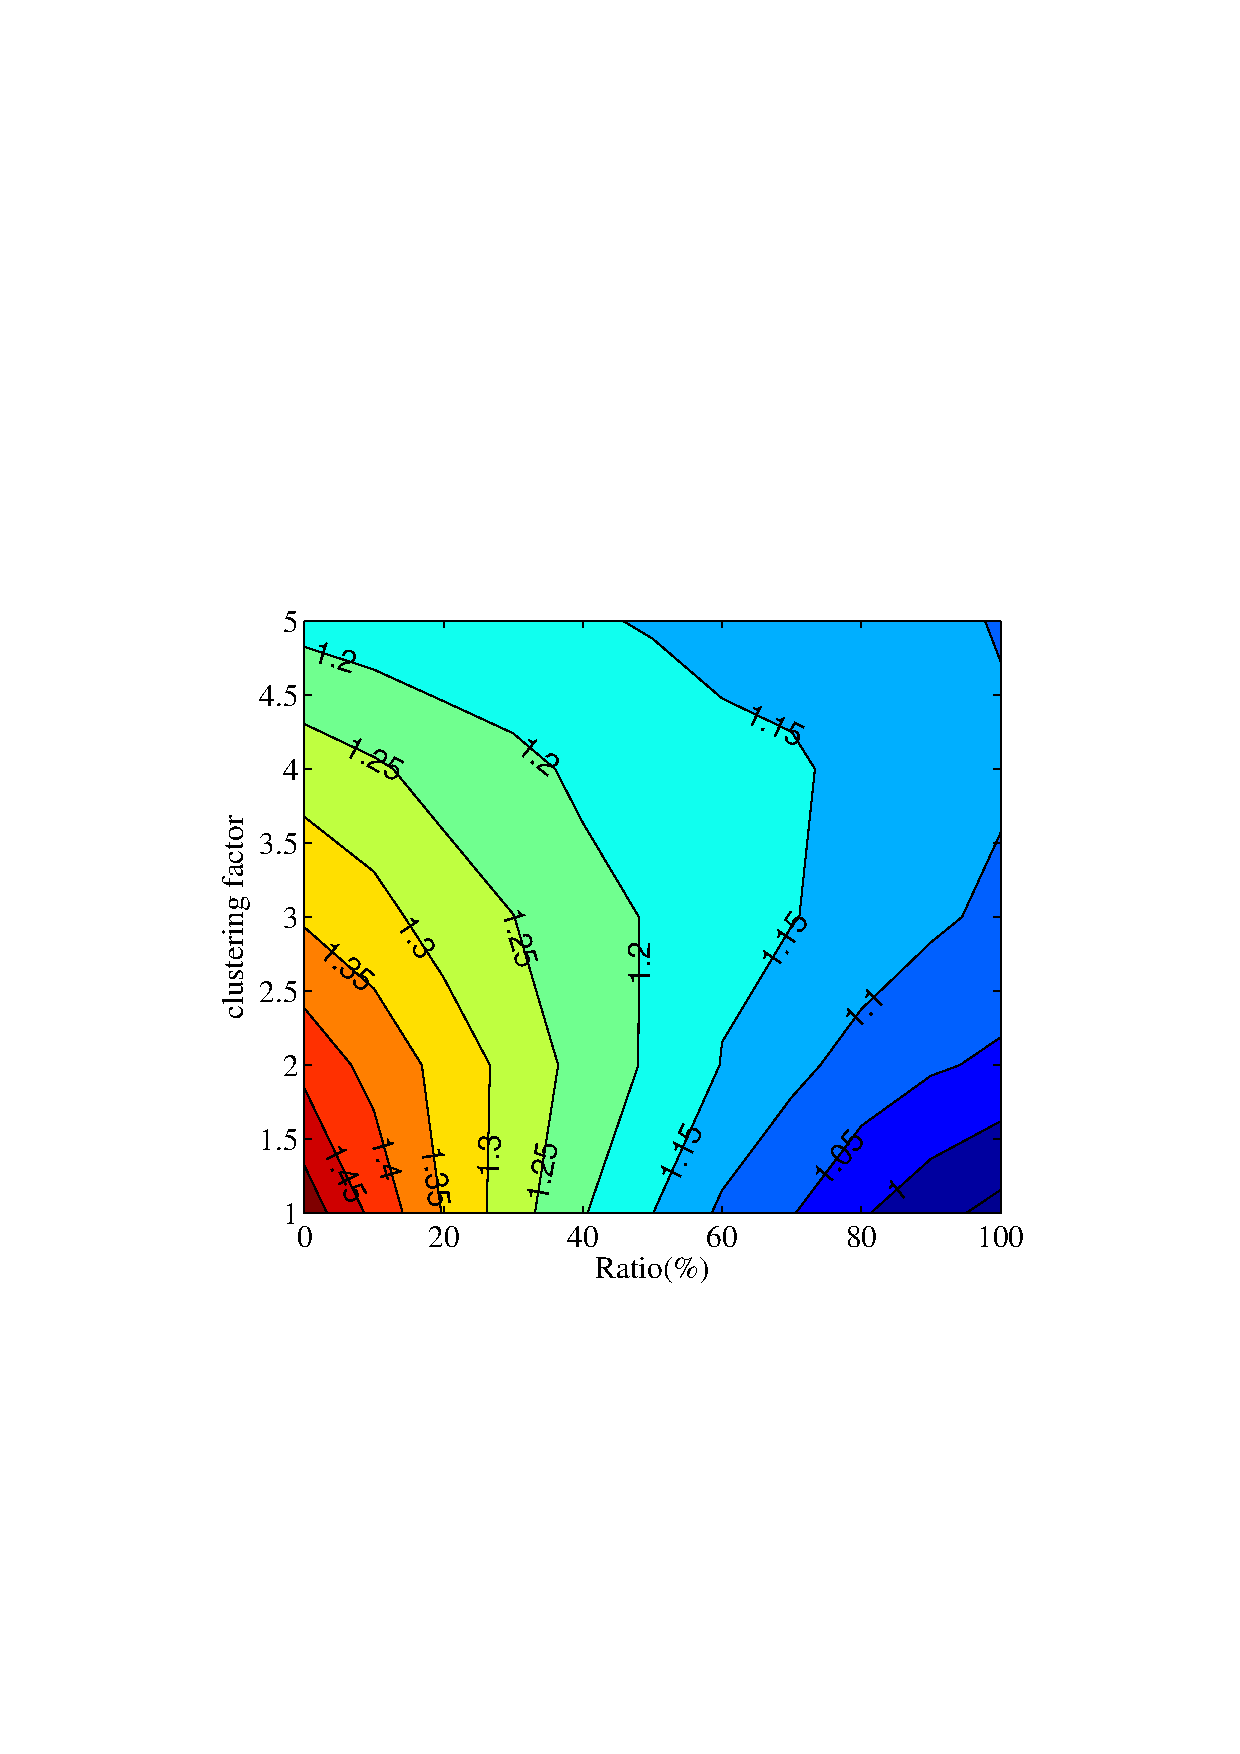
\includegraphics[width=0.8\linewidth]{figure/cfactor.pdf}
	\caption{Experiment 1: Speedup of Horizontal Clustering (HC).}
	\label{fig:shc}
	\vspace{-10pt}
\end{figure}

Experiment 2: Fig.~\ref{fig:performance} (top) shows the performance gain over HC $\mu$ of the balancing methods compared to the HC method for the LIGO workflow. HIFB and HDB significantly increase the performance of the workflow execution. Both strategies capture the structural and runtime information, reducing data transfers between tasks, while HRB focuses on runtime distribution, which in this case is none. Fig.~\ref{fig:performance} (bottom) shows the performance of the balancing methods for the Epigenomics workflow. When increasing the average data size, only HDB demonstrates significantly improvement related to HC. Investigating the structure of the Epigenomics workflow (Fig.~\ref{fig:shape}-bottom), we can see that all tasks at the same horizontal level share the same IFs ($HIFV$ = 0), because each branch (surrounded by dash lines) happen to have the same amount of pipelines. Thus, HIFB has no performance improvement when compared to HC. However, for LIGO (Fig.~\ref{fig:shape}-top), $HIFV \neq 0$, thus HIFB improves the workflow runtime performance.  
%The intuition behind this difference between HDB and HIFB is that 
HDB captures the strong connections between tasks (data dependencies) and HIFB captures the weak connections (similarity in terms of structure). In both workflows, $HDV$ is not zero thus HDB performs better than HC. 

% It is clear that with the increase of the average data size, both HDB and HIFB perform better than HRB. The reason is that both HDB and HIFB can capture the structural information and runtime information, while HRB only focuses on runtime distribution but in this case there is no runtime variance at the horizontal level. 

\begin{figure}[htb]
	\centering
	\includegraphics[width=\linewidth]{figure/exp2_ligo.pdf}
	\includegraphics[width=\linewidth]{figure/exp2_genome.pdf}
	\caption{Experiment 2: Performance of the LIGO workflow (top) and the Epigenomics workflow (bottom).}
	\label{fig:performance}
	\vspace{-10pt}
\end{figure}

Experiment 3: Fig.~\ref{fig:incluence_of_hrv} shows the performance gain $\mu$ when varying task runtimes for the LIGO workflow. As expected, when $HRV$ increases HRB over performs HC. However, HDB and HIFB demonstrate poor performance because they merge tasks based on data dependencies first, and then, they balance the runtime distribution. 
For high values of $HRV$, we just simply need to use HRB. Otherwise, we can use either HDB or HIFB while in some cases HIFB fails to capture the structural information. 

\begin{figure}[htb]
\centering
	\includegraphics[width=\linewidth]{figure/exp3.pdf}
	\caption{Experiment 3: Influence of $HRV$ (LIGO workflow).}
	\label{fig:incluence_of_hrv}
	\vspace{-10pt}
\end{figure}




\section{Sensitivity Metrics}



Many computational scientists develop and use large-scale, loosely-coupled applications that are often structured as scientific workflows, which consist of many computational tasks with data dependencies between them. When executing these applications on a multi-machine distributed environment, such as the Grid or the Cloud, significant system overheads may exist~\cite{Chen, Prodan2008b, Dong2010, Yang03, WorkflowSim} and the problem of choosing robust schedules becomes more and more important. Traditionally, a carefully crafted schedule is based on deterministic or statistic estimates for the execution time of computational activities that compose a workflow. However, in such an environment, this approach may prove to be grossly inefficient~\cite{WorkflowSim}, as a result of various unpredictable overheads that may occur at runtime. 
%Particularly, it is challenging to provide a good estimate of overheads since it involves a lot of uncertainties. 
Thus, to mitigate the impact of uncertain overheads, it is necessary to choose a schedule that guarantees overhead robustness, that is, a schedule that is affected as little as possible by various overhead changes.  

There are several ways to achieve overhead robustness. A first approach is to integrate the overhead estimation into the job scheduling problem. A static or statistic estimation of communication cost or data transfer delay~\cite{Dong2010, Yang03} has been considered in the scheduling problem. Once we have the deterministic or statistic information of overheads, we can treat the system overhead as computational activities and the goal is to minimize the overall runtime including overhead duration. However, this approach only applies to the estimation of data transfer delay since the highly unpredictable variability and variety of other overheads make it a challenging work and not efficient in practice. Our prior work~\cite{Chen} has shown the variation of overheads may be comparable to the job runtime and thus makes it unrealistic in a real environment.  

A significant amount of work~\cite{Ahmad1998, Chetto1990, Dong2010, Yang03} in the literature has focused on proposing algorithms that are aware of the dynamic changes of runtime environments. Task rescheduling~\cite{Sakellariou2004, Zhang2009, Chen2010} is a typical approach that dynamically allocates tasks to an idle processor in order to take into account information that has been made available during the execution. Specifically, resource load~\cite{Dong2010} can be used to estimate the variance. However, rescheduling a task is costly as it implies some extra communication and synchronization costs. Relevant studies~\cite{Sakellariou2004} indicate that it is important to have a static schedule with good properties before the start of the execution. Therefore, even if a dynamic strategy is used, a good initial placement would reduce the possibility of making a bad decision. 

Another approach is to overestimate the execution time of individual jobs. Delay scheduling~\cite{Zaharia10} waits for a small amount of time, letting other MapReduce jobs launch tasks instead and this method can achieve a better tradeoff of locality and fairness. However, this method only applies to workload scheduling and particularly MapReduce jobs since the duration of them is short and thus it is not difficult to estimate the scheduling delay. Also, this results in a waste of resources as it induces a lot of idle time during the execution, if the overhead is shorter than the estimation. Second, overheads do not simply work as an attachment to the job runtime and it involves a lot more complicated patterns such as periodicity~\cite{Chen}. 

In this paper, we first present our work on evaluating the overhead robustness of scheduling heuristics and we indicate a list of heuristics that are overhead robust even without an estimate of the overhead duration. Second, since the estimate of overhead duration is difficult, we develop new heuristics that leverage the pattern information of workflow overheads, which represents a new approach to design overhead robust algorithms. To the best of our knowledge, so far, no study has systematically tried to evaluate the scheduling heuristics with respect to the overhead robustness.  

%To the best of our knowledge, this study is the first example of overhead robustness of scheduling heuristics and algorithms. 
The next Section gives an overview of the related work, Section~\ref{sec:model} presents our workflow and execution environment models, Section~\ref{sec:heuristics} details our heuristics and algorithms, Section~\ref{sec:experiments} reports experiments and results, and the paper closes with a discussion and conclusions.



\section{Related Work}

Some work in the literature has attempted to define and model robustness. In~\cite{Ali2004}, the authors propose a general method to define a metric for robustness. First, a performance metric is chosen. In our case, this performance metric is the overall runtime including overhead duration as we want the execution time of an application to be as stable as possible. Second, one has to identify the parameters that make the performance metric uncertain. In our case, it is the duration of the individual overheads. Third, one needs to find how a modification of these parameters changes the value of the performance metric. In our case, the answer is, as an increase of the overhead generally implies an increase of the overall runtime. 
%Lastly, one has to identify the smallest variation of a parameter that makes the performance metric exceed an acceptable bound. 
A schedule $A$ is said to be more robust than another schedule $B$ if the variation for $A$ is larger than that for $B$.
%However, estimating this variation is the most difficult part as it requires to analyze deeply the structure of the problem and its inputs.
Following this approach, Canon~\cite{Canon2008} analyzed the robustness of 20 static DAG scheduling heuristics using a metric for robustness the standard deviation of the makespan over a large number of measurement. Braun et al. \cite{Braun2001} evaluated 11 heuristics examined and for the cases studied there, the relatively simple Min-min heuristic performs well in comparison to the other techniques. In comparison, we focus on varying the parameters related to overhead instead of computational tasks. 

A plethora of studies on task scheduling~\cite{Chetto1990, Dong2010, Yang03, Blythe2005} have been developed in the distributed and parallel computing domains. Many of these schedulers have been extended to consider both the computational cost and communication cost. A static or statistic estimation of communication cost or data transfer delay~\cite{Dong2010, Yang03} has been considered in the scheduling problem. In contrast, we focus on the scheduling overheads that have been ignored or underestimated for long and we demonstrate how their unique timeline patterns influence the overhead robustness. 

Workflow patterns~\cite{Yu2005, Juve2013, Liu2008} are used to capture and abstract the common structure within a workflow and they give insights on designing new workflows and optimization methods.  
Yu~\cite{Yu2005} proposed a taxonomy that characterizes and classifies various approaches for building and executing workflows on Grids. They also provided a survey of several representative Grid workflow systems developed by various projects world-wide to demonstrate the comprehensiveness of the taxonomy. Juve~\cite{Juve2013} provided a characterization of workflow from 6 scientific applications and obtained task-level performance metrics (I/O, CPU and memory consumption). They also presented an execution profile for each workflow running at a typical scale and managed by the Pegasus workflow management system~\cite{Deelman2005}. Liu~\cite{Liu2008} proposed a novel pattern 
based time-series forecasting strategy which ulitilizes a 
periodical sampling plan to build representative 
duration series. Compared to them, we discover a common pattern of intervals existing in system overheads while executing scientific workflows. We also leverage this knowledge to evaluate the overhead robustness of existing heuristics and develop new heuristics. 

Overhead analysis \cite{Prodan2008b}\cite{Chen} is a topic of great interest in the grid community. Stratan \cite{Stratan} evaluates workflow engines including DAGMan/Condor and Karajan/Globus in a real-world grid environment. Sonmez \cite{Sonmez} investigated the prediction of the queue delay in grids and assessed the performance and benefit of predicting queue delays based on traces gathered from various resource and production grid environments. Prodan \cite{Prodan2008b} offers a grid workflow overhead classification and a systematic measurement of overheads. Our prior work \cite{Chen} further investigated the major overheads and their relationship with different optimization techniques. In this paper, we leverage these knowledge to enhance the existing scheduling heuristics and provide insights on designing new algorithms. 

%Braun paper
%Opportunistic Load Balancing, Minimum Execution Time, Minimum Completion Time, Min-min, Max-min, Duplex, Genetic Algorithm, Simulated Annealing, Genetic Simulated Annealing, Tabu, and A*

%The 11 static mapping heuristics were evaluated using simulated execution times for an HC environment. Because these are static heuristics, it is assumed that an accurate estimate of the expected execution time for each task on each machine is known prior to execution and contained within a  ETC (expected time to compute) matrix. The assumption that these estimated expected execution times are known is commonly made when studying mapping heuristics for HC systems (e.g., [19, 26, 40]). (Approaches for doing this estimation based on task profiling and analytical benchmarking are discussed in [27, 30, 37].)

%Data dependencies between workflow tasks play an important role when clustering tasks within a level. A data dependency means that there is a data transfer between two tasks (output data for one and input data for the other). Grouping tasks without considering these dependencies may lead to data locality problems where output data produced by parent tasks are poorly distributed. Thus, data transfer times and failures probability increase.Therefore, we claim that data dependencies of subsequent tasks should be considered.




%\textbf{Workflow Management Systems} (WMS) such as Askalon \cite{Fahringer}, Taverna \cite{Oinn}, and Pegasus \cite{Deelman} are designed to run scientific workflows on distributed environments. DAGs (Directed Acyclic Graph) and other task graph representations are widely used as the programming model for many parallel applications because it is effective in expressing and optimizing irregular computations. 
%Moreover, algorithms expressed as DAGs have the potential to alleviate the user from focusing on the architectural issues, while allowing the engine to extract the best performance from the underlying architecture. 





\subsection{Overhead Patterns}

In this section, we introduce the common overhead patterns in workflow execution. 
In scientific workflow systems, time related functionalities such as workflow scheduling normally requires effective forecasting of activity patterns. In this work, we mainly focus on the overhead pattern that refers to a representative time series of overhead activities that occurs repeatedly and regularly in workflow execution. An overhead pattern is composed of ordered overhead activities obtained from scientific workflow system logs or other forms of historical data. 
Pattern discovery~\cite{Liu2008} usually starts from a periodical sampling plan to build representative duration series (Job Release, etc. ) and then conducts time-series segmentation to discover the pattern sets and predicts the activity duration intervals with pattern matching results. 


The motivation for pattern based analysis comes from the observation that for those duration-series segments where the number of concurrent activity instances is similar, these activity durations reveal comparable statistical features. Due to the dynamic nature of underlying resources, pattern based forecasting of overheads can improve the effectiveness of scheduling heuristics. 

\begin{figure}[htb]
\centering
 \includegraphics[width=1\linewidth]{figure/adherence.pdf}
  \captionof{figure}{Adherence Pattern}
  \label{fig:adhere}
  \vspace{-10pt}
\end{figure}

Most of the work~\cite{Dong2010, Yang03} view the overhead duration as an attachment to runtime in workflow timeline. For example, the Pre/Post-script Delay is usually constant, which we call it Adherence Pattern as shown in Fig.~\ref{fig:adhere}. Scheduling algorithms can just add the delay to the job runtime without significant change to the algorithms. For this pattern, we have shown in our prior work~\cite{Chen} that it does not have much influence on the overhead robustness. 
However, we observe that the Workflow Engine Delay and the Queue Delay increases periodically and steadily. For example, Fig.~\ref{fig:trace} shows the Gantt chart of part of a real trace\footnote{Details: http://www.isi.edu/\string~wchen/fgrid/run}. 
The Workflow Engine Delay (red) of the first 16 jobs is 5 seconds and then it increases to 10 seconds. 
%It is difficult to explain queue delay
We call this common overhead pattern the Incremental and Periodical Pattern (IPP). We observe the Queue Delay also increases periodically but the period is interrupted by the resource availability and thus it has a more complicated IPP. In the rest of this paper, we focus on the IPP of the Workflow Engine Delay and we will cover the Queue Delay in our future work. 
The reason why IPP prevalently exists is that many workflow management components are queue based systems. They repeatedly check their queues to find whether there are idle jobs, if yes they will process and submit these jobs, otherwise it will wait for a interval and continue. In Fig.~\ref{fig:ipp} we abstract the IPP from the trace, which shows a repeatedly increase by a interval. We define throughput of a workflow management component as the maximum number of allowed jobs in queue. For example, the interval and the throughput of the Workflow Engine in Fig.~\ref{fig:trace} are around 5 seconds and 16 respectively. 


\begin{figure}[htb]
\centering
 \includegraphics[width=1\linewidth]{figure/trace.pdf}
  \captionof{figure}{Workflow Execution Gantt Chart of a Real Trace}
  \label{fig:trace}
  \vspace{-10pt}
\end{figure}



%Some representative time series, including marketing time series, temperature time series and quality control time series, are effectively applied in various scientific and business domains [6][7]. Similarly, 

%Current forecasting strategies for computation tasks mainly reside on the prediction of CPU load [1][15], however, this is quite different from the prediction of scientific workflow activity durations.Activity durations cover the time intervals from the initial submission to the final completion of each workflow activity [3]. Hence, besides the exact execution time on scheduled resources, they also consist of extra time, i.e. scientific workflow overheads. According to [11], there exist four main categories of scientific workflow overheads, i.e. middleware overhead, data transfer overhead, loss of parallelism overhead and activity related overhead. Evidently, scientific workflow activity durations involve much more affecting factors than that of conventional computation tasks which are dominated by high performance computing resources.scientific workflow activity durations denote discrete long-term intervals since activity instances only occur occasionally and take several minutes or more than a couple of hours to complete.

%The motivation for pattern based time-series forecasting comes from the observation that for those duration-series segments where the number of concurrent activity instances is similar, these activity durations reveal comparable statistical features. 

These overhead patterns reappear frequently during a duration series and they represent unique behavior of the workflow management components. After we define and discover these typical patterns, the intervals and throughputs of these patterns can be estimated and statistically captured from historical traces. 



%Furthermore, if these overhead patterns reappear frequently during a duration series, they can be deemed as potential patterns which represent unique behavior of the duration-series under certain circumstances. Therefore, if we are able to define and discover these typical patterns, the intervals of future durations can be estimated with the statistical features of the closest patterns by matching the latest duration sequences. 





\begin{figure}[htb]
\centering
 \includegraphics[width=1\linewidth]{figure/incremental.pdf}
  \captionof{figure}{Incremental and Periodical Pattern}
  \label{fig:ipp}
  \vspace{-10pt}
\end{figure}

%It is not workflow engine delay it is workflow engine interval
\section{Overhead Robust Heuristics}
\label{sec:heuristics}
In this section, we introduce the overhead robustness of four pairs of scheduling heuristics. Heuristics are widely used in workflow scheduling since the scheduling problem is a NP-hard problem and the time complicity of a global optimization of the overall runtime is not affordable. Usually, heuristics utilize unique features of workflows or resources to guide the mapping of jobs to resources. For example, both of the MINMIN~\cite{Blythe2005} algorithm and the MAXMIN~\cite{Braun2001} algorithm utilize the runtime of a job as the feature. However, they conduct the mapping in an opposite way, that is, MINMIN chooses the job with the shortest runtime while MAXMIN chooses the job with the longest runtime. Intuitively speaking, there must be either of them (we call it overhead robust) that performs better than the other one (we call it overhead unrobust) since they operates oppositely. Inspired by these coupling heuristics, we use a relative overhead robustness approach to evaluate these scheduling heuristics. For a pair of heuristics that use the same feature, we define the relative overhead robustness as the performance gain of the overhead robust heuristic against the other one. The more performance gain we have, the more significant this feature has on the overhead robustness. Also, it is not fair to compare scheduling heuristics that use different features because they may have vastly different performance even without overheads. Furthermore, in practice, we can use scheduling heuristics with different features at the same time but not those with the same features. 
Below we introduce the four pairs of scheduling heuristics including one that we propose. 

%OLB: Opportunistic Load Balancing (OLB) assigns each task, in arbitrary order, to the next machine that is expected to be available, regardless of the task's expected execution time on that machine [3, 17, 18]. The intuition behind OLB is to keep all machines as busy as possible. One advantage of OLB is its simplicity, but because OLB does not consider expected task execution times, the mappings it finds can result in very poor makespans.
%MET: In contrast to OLB, Minimum Execution Time ( MET ) assigns each task, in arbitrary order, to the machine with the best expected execution time for that task, regardless of that machine's availability [3, 17]. The motivation behind MET is to give each task to its best machine. This can cause a severe load imbalance across machines. In general, this heuristic is obviously not applicable to HC environments characterized by consistent ETC matrices.
%MCT: Minimum Completion Time (MCT) assigns each task, in arbitrary order, to the machine with the minimum expected completion time for that task [3]. This causes some tasks to be assigned to machines that do not have the minimum execution time for them. The intuition behind MCT is to combine the benefits of OLB and MET, while avoiding the circumstances in which OLB and MET perform poorly.

\emph{MINMIN} and \emph{MAXMIN}: The MINMIN heuristic begins with a set of all unmapped jobs. Then, the set of minimum completion times for each job, M namely, is found. Next, the job with the overall minimum completion time from M is selected and assigned to the corresponding resource (hence the name MINMIN). Last, the newly mapped job is removed from the unmapped jobs, and the process repeats until all jobs are mapped. 
%Minin maps the tasks in the order that changes the machine availability status by the least amount that any assignment could. Let ti be the first task mapped by Minin onto an empty system. The machine that finishes ti the earliest, say mj , is also the machine that executes ti the fastest. For every task that MINMIN maps after ti, the Minin heuristic changes the availability status of mj by the least possible amount for every assignment. Therefore, the percentage of tasks assigned to their first choice (on the basis of execution time) is likely to be higher for Minmin than for Maxin (defined next). The expectation is that a smaller makespan can be obtained if more tasks are assigned to the machines that complete them the earliest and also execute them the fastest.
The MAXMIN heuristic is very similar to MINMIN. The MAXMIN heuristic also begins with the set of all unmapped jobs. Then, the set of minimum completion times, M, is found. Next, the job with the overall maximum completion time from M is selected and assigned to the corresponding resource (hence the name MAXMIN). Last, the newly mapped job is removed from the unmapped jobs, and the process repeats until all jobs are mapped. 
Intuitively speaking, we believe MAXMIN has better overhead robustness than MINMIN. As shown in Fig.~\ref{fig:longest}, assuming we have two jobs and the interval of the overhead is 1. MAXMIN releases a job with longer runtime first, which can overlap with the increment of the overheads when MAXMIN releases the other job. However, the performance gain depends on the values of overhead interval, job runtime, overhead duration and the resource availability. 

\begin{figure}[htb]
\centering
 \includegraphics[width=1.0\linewidth]{figure/longest.pdf}
  \captionof{figure}{MAXMIN vs. MINMIN}
  \label{fig:longest}
  \vspace{-10pt}
\end{figure}
\emph{Breadth First} and \emph{Depth First}: Namely, the Breadth First (BFS) algorithm iterates the jobs at the same workflow level (or depth within a workflow directed acyclic graph) first while the Depth First (DFS) algorithm iterates the jobs at the deepest workflow level first. Intuitively speaking, we believe BFS performs better than DFS in terms of overhead robustness since BFS releases more jobs at the same workflow level for most scientific workflows as shown in Fig.~\ref{fig:shape}. Therefore, with enough jobs in queue, BFS can fully utilize the resources without wasting this overhead interval.  

\emph{Fertile First} and \emph{Unfertile First}: The Fertile First (FFS) algorithm sorts all the unmapped jobs based on the number of children jobs that they have and assigns the jobs with most children jobs first. The Unfertile First (UFFS) algorithm works in the opposite way and assigns the jobs with lest children jobs first. Similar to the case of BFS and DFS, we believe FFS should perform better than UFFS since FFS releases more jobs at the next level compared to UFFS and thus FFS can fully utilize the available resources. 

\begin{figure}[htb]
\centering
 \includegraphics[width=0.6\linewidth]{figure/impact_factor.pdf}
  \captionof{figure}{Impact Factor}
  \label{fig:impact}
  \vspace{-10pt}
\end{figure}

\emph{Important First} and \emph{Unimportant First}: Here we propose a pair of Impact Factor based scheduling heuristics. The Important First (IFS) algorithm sorts all the unmapped jobs based on their \emph{Impact Factor} (IF) and assigns the jobs with the largest IF first while the Unimportant First (UIFS) algorithm assigns the jobs with the smallest IF first. 
The \textbf{Impact Factor} ($IF$) of a job $j_u$ is defined as follows:

\begin{equation}
	IF(j_u)=\sum_{j_v\in Child(j_u)}^{}\frac{IF(j_v)}{L(j_v)}
\end{equation}
where $Child(j_u)$ denotes the set of child jobs of $j_u$, and $L(j_v)$ the number of parent jobs of $j_v$. For simplicity, we assume the $IF$ of a workflow exit job (e.g. $j_7$ in Fig.~\ref{fig:impact}) as 1.0. For instance, consider the workflow in Fig.~\ref{fig:impact}. $IF$ for $j_1$, $j_2$, $j_3$, and $j_4$ are computed as follows:

\begin{eqnarray}
	\displaystyle  
	&IF(j_7 )=1.0, IF(j_6 )=IF(j_5 )=IF(j_7 )/2=0.5\nonumber  \\
	&IF(j_1 )=IF(j_5)/2=0.25\nonumber \\
	&IF(j_2 )=IF(j_5 )/2+IF(j_6)/3=0.42\nonumber \\
	&IF(j_3 )=IF(j_4 )=IF(j_6 )/3=0.17\nonumber 
\end{eqnarray}
Thus, IFS algorithm should schedule $j_2$ first while UIFS algorithm should schedule $j_3$ or $j_4$ first. The intuition of Impact Factor is that we aim to measure the relative importance of a job to the entire graph. Intuitively speaking, tasks with larger impact factors should have more impacts on the remaining jobs compared to tasks with smaller impact factors. For example, a bottleneck usually has a larger IF since it controls the release of more jobs. 
Similar to the case of FFS and UFFS, we believe IFS has a better overhead robustness than UIFS since IFS releases more jobs at the next few levels compared to UFFS. 


%The idea of these overhead aware heuristics is we would like to improve the overhead robustness even when we are not able to precisely predict the duration of overheads. Instead, workflow overheads have common patterns, which can determine the relative performance of different heuristics. 
Table~\ref{tab:heuristics} summaries the heuristics and their potential overhead robustness. 
\begin{table}[H]
\caption{Scheduling Heuristics}
\begin{center}
  \begin{tabular}{ l|l|l}
    \hline
Heuristics & Overhead Robust & Overhead Unrobust \\ \hline
    Experiment 1 & MAXMIN & MINMIN \\ \hline
   Experiment 2 & BFS & DFS \\ \hline
 Experiment 3 & FFS & UFFS \\ \hline
Experiment 4 & IFS & UIFS\\
    \hline
  \end{tabular}
\label{tab:heuristics}
\end{center}
\end{table}

% Section
\section{Experiment and Evaluation}
\label{sec:experiments}

The experiments presented hereafter evaluate the performance of the four pairs of heuristics mentioned ahead, which are widely used by workflow management systems. 

\subsection{Experiment Conditions}


\begin{figure}[htb]
	\centering
	\includegraphics[width=1.0\linewidth]{figure/shape.pdf} 
	\caption{A simplified visualization of the Broadband workflow, the Montage workflow and the CyberShake workflow.}
	\label{fig:shape}
	\vspace{-10pt}
\end{figure}

We extended the WorkflowSim~\cite{WorkflowSim} simulator with the overhead model to simulate a distributed environment where we could evaluate the overhead robustness of scheduling algorithms when varying the average overheads and throughput. As an initial attempt, we focus on the workflow engine delay ($d$) in this paper. The simulated computing platform is composed by 20 single core virtual machines (worker nodes), which is the quota per user of some typical distributed environments such as Amazon EC2~\cite{AmazonAWS} and FutureGrid~\cite{FutureGrid}. Each machine has 512MB of memory and the capacity to process 1,000 million instructions per second. 
%Task scheduling is data-aware, i.e. tasks are scheduled to resources which have the most input data available.
%WorkflowSim is a feature-rich toolkit to simulate workflow planning and execution. It provides runtime randomization and multiple task clustering methods that we need. 



Three workflows are used in the experiments: 
Broadband~\cite{Broadband} is an application that enables researchers to combine long-period deterministic seismograms with high-frequency stochastic seismograms. 
Montage~\cite{Sakellariou2010} is an astronomy application used to construct large image mosaics of the sky. CyberShake~\cite{Callaghan2008} is a seismology application that calculates Probabilistic Seismic Hazard curves for geographic sites in the Southern California region. All workflows are generated and varied using the WorkflowGenerator\footnote[1]{https://confluence.pegasus.isi.edu/display/pegasus/WorkflowGenerator}. Each workflow instance is composed by around 100 tasks and its workflow structure is presented in Fig.~\ref{fig:shape}. Runtime (average and task runtime distribution) and overhead (workflow engine delay and queue delay) information were collected from real traces production environments~\cite{Chen, Juve2013}, then used as input parameters for the simulations.

%We first collected runtime information  (i.e., average and distribution of task runtime) and overhead information (including workflow engine delay, queue delay and network bandwidth) from the real traces that were run on real environments before. 
%Part of runtime distribution and overhead information were shown in \cite{Juve2013} and \cite{Chen} respectively. 
%Then we input these parameters into WorkflowSim and run these workflows repeatedly until the variance is less than 5\% of the average workflow runtime. 



Four sets of experiments are conducted. Experiment 1 evaluates the relative robustness of MAXMIN and MINMIN by comparing the performance gain of the overhead robust heuristic (MAXMIN in this experiment) over the overhead unrobust heuristic (MINMIN), while varying the average interval of workflow engine ($d$) and throughput of workflow engine ($t$). Table~\ref{tab:heuristics} shows the heuristics compared in these experiments. Simulation results present a confidence level of 95\%. Thus, for values of \emph{Performance Gain} $> 0$, the overhead robust heuristics perform better than the respective overhead unrobust heuristics. Otherwise, the overhead robust heuristics perform poorer.
%We randomly select 20\% from LIGO workflow tasks and increase their task runtime by a factor of \emph{Ratio} to simulate the system variation in a production environment.




In these experiment sets, we vary the average throughput of workflow engine from 1 to 20 and we show the results of $t=1, 5, 15, 20$. The original throughput of workflow engine in these traces is 5 and a throughput that is larger than 20 does not influence the performance much since we have only 20 worker nodes in our experiments. We also vary the average interval of workflow engine from 0 to 100 seconds, which represents a typical range of workflow engine delay as shown in~\cite{Chen} and this range is able to show the difference of overhead robustness in these heuristics. 

\subsection{Results and Discussion}

\begin{figure}[!htb]
\centering
 \includegraphics[width=0.9\linewidth]{figure/MAX-MIN-Broadband.pdf}
  \captionof{figure}{Broadband }
  \label{fig:MAX-MIN-Broadband}
  \vspace{-10pt}
\end{figure}

\begin{figure}[!htb]
\centering
 \includegraphics[width=0.9\linewidth]{figure/MAX-MIN-CyberShake.pdf}
  \captionof{figure}{CyberShake}
  \label{fig:MAX-MIN-CyberShake}
  \vspace{-10pt}
\end{figure}

\begin{figure}[!htb]
\centering
 \includegraphics[width=0.9\linewidth]{figure/MAX-MIN-Montage.pdf}
  \captionof{figure}{Montage}
  \label{fig:MAX-MIN-Montage}
  \vspace{-10pt}
\end{figure}


Experiment 1: Fig.~\ref{fig:MAX-MIN-Broadband},~\ref{fig:MAX-MIN-CyberShake},~\ref{fig:MAX-MIN-Montage} show the  \emph{Performance Gain} of MAXMIN over MINMIN for the three workflows. We expected to see most  \emph{Performance Gain} $>0$ if MAXMIN is a overhead robust heuristic compared to MINMIN. However, except for the Montage workflow, the \emph{Performance Gain} is not significant for all of parameter settings, which concludes that MAXMIN is not globally overwhelming MINMIN in terms of overhead robustness. The reason we believe is that the  \emph{Performance Gain} in this comparison highly depends on the ratio of job runtime, workflow engine delay, number of resources and throughput of workflow engine. 

\begin{figure}[!htb]
\centering
 \includegraphics[width=0.9\linewidth]{figure/DFS-BFS-Broadband.pdf}
  \captionof{figure}{Broadband }
  \label{fig:DFS-BFS-Broadband}
  \vspace{-10pt}
\end{figure}

\begin{figure}[!htb]
\centering
 \includegraphics[width=0.9\linewidth]{figure/DFS-BFS-CyberShake.pdf}
  \captionof{figure}{CyberShake}
  \label{fig:DFS-BFS-CyberShake}
  \vspace{-10pt}
\end{figure}

\begin{figure}[!htb]
\centering
 \includegraphics[width=0.9\linewidth]{figure/DFS-BFS-Montage.pdf}
  \captionof{figure}{Montage}
  \label{fig:DFS-BFS-Montage}
  \vspace{-10pt}
\end{figure}


Experiment 2: Fig.~\ref{fig:DFS-BFS-Broadband},~\ref{fig:DFS-BFS-CyberShake},~\ref{fig:DFS-BFS-Montage} show the \emph{Performance Gain} of BFS over DFS for the three workflows. We observe that most  \emph{Performance Gain} $>0$ and thus BFS performs better than DFS in terms of overhead robustness. What is more, Fig~\ref{fig:DFS-BFS-CyberShake} shows with the increase of average throughput, the \emph{Performance Gain} is more significant. We can also see that when the average throughput is high, the \emph{Performance Gain} increases with the average interval of workflow engine. This suggests us in a real environment with a large overhead, we should use BFS instead of DFS. 


\begin{figure}[!htb]
\centering
 \includegraphics[width=0.9\linewidth]{figure/UFFS-FFS-Broadband.pdf}
  \captionof{figure}{Broadband }
  \label{fig:UFFS-FFS-Broadband}
  \vspace{-10pt}
\end{figure}

\begin{figure}[!htb]
\centering
 \includegraphics[width=0.9\linewidth]{figure/UFFS-FFS-CyberShake.pdf}
  \captionof{figure}{CyberShake}
  \label{fig:UFFS-FFS-CyberShake}
  \vspace{-10pt}
\end{figure}

\begin{figure}[!htb]
\centering
 \includegraphics[width=0.9\linewidth]{figure/UFFS-FFS-Montage.pdf}
  \captionof{figure}{Montage}
  \label{fig:UFFS-FFS-Montage}
  \vspace{-10pt}
\end{figure}



Experiment 3: Fig.~\ref{fig:UFFS-FFS-Broadband},~\ref{fig:UFFS-FFS-CyberShake},~\ref{fig:UFFS-FFS-Montage} show the \emph{Performance Gain} of FFS over UFFS for the three workflows. We observe that most  \emph{Performance Gain} $>0$ and thus FFS performs better than UFFS in terms of overhead robustness, which is similar to Experiment 2. Comparing Fig.~\ref{fig:DFS-BFS-Broadband} and Fig.~\ref{fig:UFFS-FFS-Broadband} we can see the \emph{Performance Gain} of FFS over UFFS is more significant (30\%) than that of BFS over DFS (20\%).  
\begin{figure}[!htb]
\centering
 \includegraphics[width=0.9\linewidth]{figure/UIFS-IFS-Broadband.pdf}
  \captionof{figure}{Broadband }
  \label{fig:UIFS-IFS-Broadband}
  \vspace{-10pt}
\end{figure}

\begin{figure}[!htb]
\centering
 \includegraphics[width=0.9\linewidth]{figure/UIFS-IFS-CyberShake.pdf}
  \captionof{figure}{CyberShake}
  \label{fig:UIFS-IFS-CyberShake}
  \vspace{-10pt}
\end{figure}

\begin{figure}[!htb]
\centering
 \includegraphics[width=0.9\linewidth]{figure/UIFS-IFS-Montage.pdf}
  \captionof{figure}{Montage}
  \label{fig:UIFS-IFS-Montage}
  \vspace{-10pt}
\end{figure}
Experiment 4: Fig.~\ref{fig:UIFS-IFS-Broadband},~\ref{fig:UIFS-IFS-CyberShake},~\ref{fig:UIFS-IFS-Montage} show the \emph{Performance Gain} of IFS over UIFS for the three workflows. We observe that most  \emph{Performance Gain} $>0$ and thus IFS performs better than UIFS in terms of overhead robustness, which is similar to Experiment 3. The reason is that for these workflows, IF based heuristics can produce similar schedule as the heuristics based on the number of children. Most of the workflows used in this paper is not irregular enough and thus we are not able to show the difference of IF based heuristics and the heuristics based on the number of children. 

%% References with bibTeX database:

\bibliographystyle{elsarticle-num}
\bibliography{biblio}

%% Authors are advised to submit their bibtex database files. They are
%% requested to list a bibtex style file in the manuscript if they do
%% not want to use elsarticle-num.bst.

%% References without bibTeX database:

% \begin{thebibliography}{00}

%% \bibitem must have the following form:
%%   \bibitem{key}...
%%

% \bibitem{}

% \end{thebibliography}


\end{document}

%%
%% End of file `elsarticle-template-num.tex'.
